\documentclass[ProjectABM]{subfiles}
% WARNING: AuCTeX local variables only get reset when file is loaded
% and differ between this file and ProjectABM.tex
% so must re-load whichever file you want to compile with C-x C-v

% WARNING: Different AucTeX execution depending on whether
% 0. Being compiled as standalone document
%    * Compile main once
%    * Then compile this one
%    * Keep compiling until nothing changes
% 0. Being compiled as subfile of main document
%    * Just compile main document repeatedly

\providecommand{\econtexRoot}{}
\renewcommand{\econtexRoot}{..}
\providecommand{\econtexPaths}{}\renewcommand{\econtexPaths}{\econtexRoot/Resources/econtexPaths}
% The \commands below are required to allow sharing of the same base code via Github between TeXLive on a local machine and Overleaf (which is a proxy for "a standard distribution of LaTeX").  This is an ugly solution to the requirement that custom LaTeX packages be accessible, and that Overleaf prohibits symbolic links
\providecommand{\econtex}{\econtexRoot/Resources/texmf-local/tex/latex/econtex}
\providecommand{\econtexSetup}{\econtexRoot/Resources/texmf-local/tex/latex/econtexSetup}
\providecommand{\econtexShortcuts}{\econtexRoot/Resources/texmf-local/tex/latex/econtexShortcuts}
\providecommand{\econtexBibMake}{\econtexRoot/Resources/texmf-local/tex/latex/econtexBibMake}
\providecommand{\econtexBibStyle}{\econtexRoot/Resources/texmf-local/bibtex/bst/econtex}
\providecommand{\econtexBib}{economics}
\providecommand{\notes}{\econtexRoot/Resources/texmf-local/tex/latex/handout}
\providecommand{\handoutSetup}{\econtexRoot/Resources/texmf-local/tex/latex/handoutSetup}
\providecommand{\handoutShortcuts}{\econtexRoot/Resources/texmf-local/tex/latex/handoutShortcuts}
\providecommand{\handoutBibMake}{\econtexRoot/Resources/texmf-local/tex/latex/handoutBibMake}
\providecommand{\handoutBibStyle}{\econtexRoot/Resources/texmf-local/bibtex/bst/handout}

\providecommand{\FigDir}{\econtexRoot/Figures}
\providecommand{\CodeDir}{\econtexRoot/Code}
\providecommand{\DataDir}{\econtexRoot/Data}
\providecommand{\SlideDir}{\econtexRoot/Slides}
\providecommand{\TableDir}{\econtexRoot/Tables}
\providecommand{\ApndxDir}{\econtexRoot/Appendices}

\providecommand{\ResourcesDir}{\econtexRoot/Resources}
\providecommand{\rootFromOut}{..} % Path back to root directory from output-directory
\providecommand{\LaTeXGenerated}{\econtexRoot/LaTeX} % Put generated files in subdirectory
\providecommand{\econtexPaths}{\econtexRoot/Resources/econtexPaths}
\providecommand{\LaTeXInputs}{\econtexRoot/Resources/LaTeXInputs}
\providecommand{\LtxDir}{LaTeX/}
\providecommand{\EqDir}{Equations} % Put generated files in subdirectory


\onlyinsubfile{% https://tex.stackexchange.com/questions/463699/proper-reference-numbers-with-subfiles
    \csname @ifpackageloaded\endcsname{xr-hyper}{%
      \externaldocument{\econtexRoot/BufferStockTheory}% xr-hyper in use; optional argument for url of main.pdf for hyperlinks
    }{%
      \externaldocument{\econtexRoot/BufferStockTheory}% xr in use
    }%
    \renewcommand\labelprefix{}%
    % Initialize the counters via the labels belonging to the main document:
    \setcounter{equation}{\numexpr\getrefnumber{\labelprefix eq:Dummy}\relax}% eq:Dummy is the last number used for an equation in the main text; start counting up from there
}


\onlyinsubfile{\externaldocument{ProjectABM}} % Get xrefs -- esp to appendix -- from main file; only works properly if main file has already been compiled;

\begin{document}

% Attempted to make all lines used for Web version contain {Web} (or version with only single curly brace at end) so can be removed with sed
\providecommand{\versn}{pdf} % Version; like, web or pdf or journal submission
\ifthenelse{\boolean{Web}}{    % {Web}
  \renewcommand{\versn}{Web}     % Too hard to figure out passing -output-directory through make4ht through htlatex, so web version is compiled with junk files in main directory
  \renewcommand{\rootFromOut}{.} % {Web}
}{}  % {Web}

% Tiny info header at top to track git commit
%\hfill{\tiny \jobname~\versn~\today~{at} \DTMcurrenttime, \input{\ResourcesDir/.git-source-commit}~~\input{\ResourcesDir/.git-public-commit}}

\title{Equity Premium Puzzle, Expectations and Covid-19:\\ Evidence from Germany}

\author{Adrian Monninger\authNum}

\keywords{equity premium puzzle - participation cost - adjustment costs - expectations - covid19}

\jelclass{D14, G11, G5}


\renewcommand{\forcedate}{October 14, 2021}\date{\forcedate}

\maketitle
\hypertarget{abstract}{}
\begin{abstract}
This paper uses information from the Bundesbank Online Pilot Survey on Consumer Expectations (BOP) wave 8 and compares various mechanisms why households do not hold stocks, what prevents them from adjusting their portfolio, and what makes them overcome them. My results are \textcolor{orange}{results}.
\end{abstract}


% Various resources
\hypertarget{links}{}

\begin{authorsinfo}
  \name{Contact: \href{mailto:amonnin1@jhu.edu}{amonnin1@jhu.edu} }, Department of Economics, 590 Wyman Hall, Johns Hopkins University, Baltimore, MD 21218, 
\end{authorsinfo}

\newcommand{\thankstext}{
I am deeply indebted to the members of the Deutsche Bundesbank BOP team, in particular Tobias Schmidt, Stefan Ried, Olga Goldfayn-Frank and Misina Cato, as well as Chris Carroll, Annette Vissing-Jorgensen and my fellow students from the Johns Hopkins University. All errors are my own.}

\ifthenelse{\boolean{Web}}{}{
  \begin{minipage}{0.9\textwidth}
    \tiny \thankstext
\end{minipage}
} % {Web}
{\titlepagefinish}

\hypertarget{Introduction}{}
\section{Introduction}\label{sec:intro}

\paragraph{Many theories to explain equity premium puzzle}
The equity premium puzzle is not a new phenomenon, but a vibrant one. Household finance papers have tested empirically a variety of factors why households do not hold stocks at all and if they do, why such a small share of their portfolio.

\paragraph{This paper: high level summary}
These factors are usually tested one by one using different time periods, locations, and reference groups which makes a comparison almost impossible. This paper uses data from the Bundesbank Online Panel (BOP) and asks around 2000 households to assess factors which played a role in their financial investment decision. %\textit{What are the most important factors of the equity premium puzzle?} With the natural follow up question \textit{And what makes households overcome them?}

\paragraph{Contributions:}
The contributions of this paper are threefold. Firstly, I can compare the importance of many factors and assess how they correlate with each other. Secondly, while most papers focus on the participation part, I ask why households did not adjust their portfolio, or if they did what drove their decision. Lastly, I can link financial asset investment decisions with expectations about macro-variables.

% \begin{itemize}
	%     \item Asking directly many mechanisms
	%     \item Not only participation, but why bought, sold, not adjust
	%     \item Expectations: Not only about stock market expectation, but other macro variables
	% \end{itemize}

\paragraph{My Results}
\begin{enumerate}
	\item No participation:
	\begin{itemize}
		\item lack of information and interested most important, before risk factors
		\item 3 components: risk aversion, lack of resources, no savings
		\item first 2 lifecycle component, last income component
	\end{itemize}
	\item No Adjustment
	\begin{itemize}
		\item Market is too risky/uncertain atm
		\item 2 components: bad timing and lack of time
		\item needs to get further attention
	\end{itemize}
	\item Bought
	\begin{itemize}
		\item Good starting point or had a savingsplan in place
		\item First time buyers: more time
		\item Bought same asset type
	\end{itemize}
	\item Sold
	\begin{itemize}
		\item cash out or rebalancing
		\item some are driven out
	\end{itemize}
	\item Expectations
	\begin{itemize}
		\item Houseprices crowd out financial asset investments (Owner and renter)
		\item Higher inflation expectations reduces likelihood to buy
	\end{itemize}
\end{enumerate}
% \begin{itemize}
	%     \item 50\% no participation, 25\% participated, but did not adjust and 25\% adjusted their portfolio.
	%     \item Demographics which increased the probability to buy stocks are: education (college graduates), sex (male), wealth (higher income), age (being younger than 30)
	%     \item Reasons no participation: 70\% agree that lack of information and no interest is important, 60\% distrust, time constraints and peer-effects
	%     \item By demographics: variation can be captured by cohort effects; female are less interested
	%     \item Reasons un-adjusted: too risky, high valuation and no time most important
	%     \item By demographics: no additional savings and peer-effect captured by cohort effects. The three above are relatively constant
	%     \item Reason bought: low valuation and saving plan are very important
	%     \item first time buyers: time played a role
	%     \item bought and sold: low valuation and additional information, but less likely a savings plan
	%     \item Reason sold: high valuation and re-balancing most important, some sold due to uncertainty and shock
	%     \item Buy asset types: fonds and bonds most prominently held. Re-balancing from fonds towards bonds. Mostly bought asset type they already held
	%     \item Buy and Expectations: more likely to buy if think gdp increases stronger and lower if property prices increase stronger. Counter-intuitively, probability increases when unemployment is expected to increase %could be due to: If updated expectations on any variable, more likely to buy: Updating and additional information effect. Could hold for unemployment rates as well (was heavily in the news)
	% \end{itemize}

% No insights in:
% \begin{itemize}
	%     \item Value bought (tried, reg, tobit, heckman); also ratio income not much. Might be something with reasons (low valuation and more income is important, plan and time not)
	% \end{itemize}


%\paragraph{Equity premium puzzle}

\paragraph{Why 2020?}
The year 2020 is an interesting time period to study. Due to covid-19 restrictions in March 2020, stock market prices plummeted by \textbf{X\%} and recovered to \textbf{X\%} by \textbf{XXXX}. Nevertheless, the overall participation rate increased. The DAI reports that 2.7 mio additional people held stocks compared to 2019. Here, the biggest increase (40\%) was made for Germans younger than 40. \textbf{Add PAPI if ready}

% DAI 2021: 
% \begin{itemize}
	%     \item 12.4 mio people own financial assets/ 1/6 above 14
	%     \item in 2020: 
	%     \begin{itemize}
		%         \item 2.7mio more
		%         \item 1 mio younger than 40
		%         \item 14-29 years: +67\%
		%         \item 30-39 years: +34\%
		%         \item <40: +40\%
		%     \end{itemize}
	% \end{itemize}

% Add numbers of other countries?!

Economic theory gives many explanations how this period impacts financial investment decisions. Firstly, \cite{malmendier_2011} would argue that the vast decline in stock prices scares people away. Additionally, the path of recovery contains a lot of uncertainty. Do covid-cases decrease soon, will there be a vaccine available, or additional mutants which worsens the situation again? All this is reflected in the stock market, hence, \textbf{CAPM?} suggests that people would reduce their asset holdings.

On the contrary, the bufferstock model by \textbf{Carroll} suggests that higher uncertainty leads to higher savings. As background risks such as income risks increased as well, households would like to save to dampen possible shocks. %While it is not clear, whether households should invest in the stock market, it is definetely one possibility. 
Additionally, past experiences suggest that after a crash, there will be a recovery and hence, the crisis could mark a good opportunity to start investing. Lastly, covid affected everyday life in many dimensions. Consumption restrictions could have increased savings and free time for some households. Of course, this experience is extremely heterogeneous, as working remotely and home schooling increased not only the need for digital infrastructure, but also marked a huge burden on families with small children.

% This increase can have many sources. 
% LITERATURE SUMMARY ABOUT FACTORS RELEVANT IN 2020

% Covid-19 affected everyday life and the economy in many dimensions. Firstly, after restrictions in March 2020, stock market prices fell vastly. \cite{malmendier_2011} would argue that this experience scares people away

% \begin{itemize}
	%     \item Show graphs of stockholding puzzles (HFCS, SCF)
	%     \item Show fall and sore of stock markets after Corona (compare with 2008?) 
	% \end{itemize}
% Stories:
% a) Factors which could decrease stock holdings: 
% i) shock: scared people away (Malmendier and nagel)
% ii) Which recovery? V,L,W,K? Leads to higher uncertainty

% b) Factors which could increase stock holdings:
% i) Higher uncertainty leads to higher savings (Bufferstock Carroll)
% ii) After crises low valuation which makes it a good opportunity to invest
% iii) Covid specific factors: consumption restrictions (more savings for some) and more time (for some)



% \paragraph{My research question}

% \paragraph{My Data}



\paragraph{Data + Survey Methodology}
This richness of mechanisms makes it nearly impossible to identify each factor individually. Therefore, I ask respondents directly which factors played a bigger role and which did not in their decision process. The BOP asks a representative sample of 2000 German households on a monthly basis. Next to demographics and expectations of macro-variables as well as personal income or consumption dynamics, I included 5 to 6 questions for each respondent. They investigate the main drivers of financial decisions based on each type. Between March 2020 (the beginning of corona restrictions) and August (when the interview took place), respondents could have either i) not participated ii) not adjusted, iii) bought additional assets or iv) sold assets. Each type receives a set of questions where they need to rank each possibility.

Asking households directly are appealing in this context to compare the mechanisms, but have weaknesses. \textbf{ADD THEM HERE: PROS AND CONS}

% \cite{choi_2020}: 'Survey methodologies, of course, have weaknesses. Survey respondents might not be highly motivated to give accurate responses, and the meaning of each response category (e.g., “very important”) probably differs across respondents. However, to the extent that such measurement error is white noise, the ordinal ranking of importance and agreement ratings will still be informative.More fundamentally, individuals might not know the true motivations for their decisions because they have not introspected seriously enough, their memory has faded, or they were subliminally influenced. A related critique is the argument that respondents may not regard a factor as important but nonetheless invest “as if” it were (Friedman (1953)). Under this view, the fact that an assumption is false is unimportant as long as it generates accurate predictions.' \textbf{Methodology: Survey Weaknesses}

% \cite{choi_2020}: '1. perceptions are unlikely to be entirely unrelated to true decision-making process 2. choose between theories that have similar predictions for prices and quantities but very different implications for our understanding of the world 3. individuals’ perceptions of their decision-making process affect how they forecast their future actions, which itself is an input into their actions today 4. these perceptions can affect an individual’s demand for debiasing mechanisms, information, and advice 5. we believe that it is inherently interesting to know what individuals believe about themselves and the reasons for their behavior. Barberis et al. (2015) argue that theory should endeavor to match survey measures of investor beliefs.' \textbf{Why surveys are a good idea}

\paragraph{Rest of Paper}
The rest of the paper is structured as follows. First, Section \ref{sec:literature} summarizes drivers of financial decisions as well as household expectations. Afterwards, section \ref{sec:data} discusses the questionnaire as well as descriptions of the data. If you are just interested in results, you can forward to section \ref{sec:results}. Lastly, section \ref{sec:robustness} assesses generality of the results and section \ref{sec:discussion} discusses them.

%\hypertarget{The-Problem}{}

\section{Literature Review}\label{sec:literature}

\paragraph{Intro}
This paper builds upon two large literature strands. The equity premium puzzle and the growing expectations literature.

\paragraph{Equity Premium puzzle in general}
The equity premium puzzle describes the fact that the difference between stock market returns and riskfree rate cannot be explained with macroeconomic models using \textit{reasonable numbers} for relative risk aversion parameters (See \cite{mehra_porescott_1985equity_premium, haliassos_bertraut_1995equity_premium, Gomes_et_al_2021}).\footnote{ The actual size depends on measurement, time and space (see\cite{vanEwijk_et_al_2012meta_equity_premium} for a meta analysis)}. The equity premium puzzle is twofold. First, the low participation in the stock market and second, the relative low share of assets invested in the stock market (\cite{campbell_2006household_finance}). 
The literature can be grouped in three categories: risks, participation costs, and social interaction.

\paragraph{Risk}
One explanation focuses on risks of households. Especially, the correlation between labor income and stocks can limit participation (e.g.,\textbf{ Benzoni, Collin-Dufresne, and Goldstein (2007))} \textbf{OTHER BACKGROUND RISKS SUCH AS HEALTH, HOUSING}
When it comes to stock market volatility, \cite{malmendier_2011} argue that experiencing macroeconomic shocks can have long lasting effects on financial risk taking behavior and find evidence in the US. A similar study by \cite{ampudia_ehrmann_2017macroeconomic} uses European data confirms the results. 
Additionally, a macroeconomic shock can also increase uncertainty in the period after the shock occurred. Basic economic models argue that an increase in volatility, should decrease the savings households put in the stock market. \textbf{CAPM?}

\paragraph{Participation Costs}
Early models such as \cite{vissing_2003} \textbf{Haliassos and Michaelides (2003), and Gomes and Michaelides (2005)} impose a small participation cost to match empirical moments. As not everyone has the same resources, only a fraction of households will participate in equity markets. While direct costs such as setting up a brokerage account only makes a small part of it, a large literature explores indirect costs.

\paragraph{Information/Financial Literacy}
The first big bulk focuses on information costs. \cite{king_leape_1987asset} uses the Survey of Consumer Financial Decisions and show that more than one third of non-participants argue that 'they did not know enough about it' as a reason of their non-participation. These can consist of unawareness of financial products such as different stocks and funds and financial literacy. For the former \cite{guiso_jappelli_2005} finds that soecioeconomic variables such as education, wealth, income, year of birth, as well as long-term bank relations, social interaction and newspaper readership increases the awareness which then increases the probability of stock market participation. Information issues appear through financial illiteracy. \cite{lusardi_mitchell_2011financial_literacy} show that many households lacking knowledge of basic principles. In an overview, they report that women are less financially literate -- which leads to lower stock holding participation (\cite{almenberg_2015gender}) -- and higher educated are also more financial literate. Additional factors are ethnic/racial and regional differences. Several papers show the strong link between financial literacy and stock market participation. For instance, \cite{guiso_japelli_2002household_book} use Italian data, \cite{hochguertel_et_al_2002household,vanrooij_et_al_2011} Dutch and \cite{borsch_eymann_2000household} German data.

\paragraph{no interest}
Another factor is that households are not interested in the stock market. This ''financial anxiety'' or ''financial phobia'' (\cite{shapiro_burchell_2012}) is an often overlooked factor. \cite{choi_2020} show that in the US 37\% of nonparticipants stated that 'not liking to think about one's finances' was a very or extremely important factor of their non-stock holding.

\paragraph{Time}
Lastly, gathering information, making the decision, and implementing it takes time. \cite{bonaparte_et_al_2012adjustment} models it as a proportion of income to capture opportunity costs. \cite{choi_2020} finds that time constraints play only a factor for 3\% of nonparticipants in their sample. %Nevertheless, this factor might not be easy to capture in survey questions.

%\cite{choi_2020}: 'Second, we ask about the importance of having intended to invest in stocks but simply not having gotten around to it (''intended to invest in stocks but never got around to it''), perhaps due to tie-inconsistent procrastination (Laibson (1997), O'Donoghue and Rabon (1999))'. \textbf{Time}

%\cite{choi_2020}: 'the lest important factor is delay despite an intention to invest in stock (3\% of nonparticipants). Prior evidence shows that individuals' financial choices exhibit considerable inertia (Samuelson and Zeckhauer (1988), Choi et al. (2002, 2004)), but people do eventually move away from their status quo to what they perceive to be their optimum (Carroll et al. (2009)), even if it takes them a few years. Therefore, in a sample that includes many middle-aged and older adults, it may not be unexpected that procrastination is a relatively small determinant of stock market nonparticipation.' \textbf{Time}


%Adjustment Cost
%In addition to participation costs, households face adjustment costs when they change their portfolio. Models without them tend to match participation rates, but predict a portfolio share in financial assets of close to 100\% (Coco and Gomes?). \cite{bonaparte_et_al_2012adjustment} models them solely as a proportion of income, but the literature on assessing it empirically is scarce.

%\cite{bonaparte_et_al_2012adjustment}: 'the cost of trading stocks takes a particular form: a proportion of income. As noted, this captures a time cost of trading' \textbf{Time and Adjustment} $\to$ should the reason increase importance with income? Alternatively: if richer, more likely to have some advisor...

\paragraph{Trust/Sociability/Peer Effect}
%\cite{georgarakos_pasini_2011} summarizes another channel regarding trust and sociability. 
Trust is studied by \cite{guiso_et_al_2008trusting} who show that households with lower trust in other people are more afraid of being cheated on which lowers the expected payoffs from stock holdings.
The second channel connects stock market participation with social interaction and peer-effects (e.g. \cite{georgarakos_pasini_2011, brown_2008, hong_et_al_2004social}). The mechanism is that gaining information is costly and "word-of-mouth" communication can lower these costs (\cite{brown_2008}). Another possibility is stated in \cite{hong_et_al_2004social} and argues that individuals have pleasure in discussing up and downs of stock markets as casual conversation topic. Examples of these effects on stock market behavior are plenty and consist of parental transmission \textbf{(Chiteji and Stafford (2000))}, workplace \textbf{(Duflo and Saez (2002))}, neighbors and church communities (\cite{hong_et_al_2004social, brown_2008}, among others.
Following \cite{georgarakos_pasini_2011} who uses the classification by \textbf{Durlauf and Fafchamps' (2004)}, the difference between the two is that interpersonal trust, sharing and reciprocity, while the latter focuses social networks or civic engagement.

% \paragraph{Personal Values/Moral}
% Lastly, personal values or moral issues can prevent households from holding stocks. \cite{kaustia_2011} argue that personal values determine investment decisions and individuals have a taste for different investment goods (similar to consumption goods). While this can just lead to a preferred asset type, 'stock market aversion' can also appear due to a cognitive dissonance between personal values and actions. Hence, individuals might not want to invest.

\paragraph{Expected Return Beliefs and Stock Market Participation}
The second class of literature focuses on expectations of traders/ households and their financial asset investments. \cite{arrondel_et_al_2014subjective_return_expectation} finds that participation increases monotonically with stock market expectations. \cite{giglio_et_al_2019five} finds empirical evidence for retail investors and \cite{choi_2020} shows that expected higher returns are very or extremely important by a quarter of all stock market participants.

\textbf{TBD: ADD OTHER PAPERS}

\paragraph{Gap In the Literature}
This paper contributes to three gaps in the literature. First, it compares magnitudes or importance of participation costs. Here, it is close to \cite{choi_2020} who asks around 1000 household heads what their portfolio equity share determines. One important difference to this paper is that while they ask for \textit{general factors}, I focus on reasons concerning a fixed 6 months period which makes it more concrete. Other papers such as \cite{bender_et_al_2019} focus on wealthy investors

Second, adjustment costs which need to be paid when changing the portfolio haven't received much attention even though they are crucial when matching not only participation, but portfolio shares invested in equity markets. \cite{bonaparte_et_al_2012adjustment} model them solely as a proportion of income, but do not give empirical evidence. In this paper, I ask households for reasons why they did not adjust their portfolio, as well as, why they adjusted it.

Thirdly, papers on expectations focus solely on expected stock market returns and stock market investments. Here, I shift attention towards stock market participation and other macro-variables such as inflation and house prices.


\section{Data}\label{sec:data}

The data source of this paper is the \textit{'Bundesbank Online Pilot Survey on Consumer Expectations'}\footnote{This paper uses data from the Bundesbank Online Pilot Survey on Consumer Expectations. The results published and the related observations and analysis may not correspond to results or analysis of the data producers.}, which is a monthly survey conducted by the Deutsche Bundesbank since April 2020\footnote{The pilot phase covers the months April to June 2019, see \cite{bundesbank_2020} for details.}. A representative sample of around 2000 German households per wave report their expectations about the development of inflation, house prices and interest rates in Germany as well as their past and planned expenditures and socio-demographic characteristics. In addition to questions which are asked on a regular basis, each wave has room for specific research questions.

\subsection{Key Variables}
In wave 8 (August 2020), households were asked three to six questions regarding their stock market behavior\footnote{The complete questionnaire can be found in the appendix \ref{App_Questionnaire} or at the Bundesbank website.}. Figure \ref{fig:timeline} shows the time line of the questions. Firstly, respondents are asked if they held any financial assets (stocks, bonds, funds, others\footnote{The questionnaire contains info boxes about each asset type.}) actively in their portfolio prior the covid-19 pandemic. In case one of these questions is affirmed, the amount can be selected as a categorical variable. Secondly, I document their behavior between March and August. Here, respondents report whether they bought, sold or left their portfolio unchanged with a follow up question about the market value of these changes. %\textcolor{orange}{Reasons for this 6 month period only! Others eg \cite{choi_2020} does ask factors in general. Time bias (what is actually important and what used to be important) or what you think used to be important in the past. Also no savings or no time can be quiet seasonal. Same for shocks (its the corona shock) and the 2020 uncertainty...}

Based on the answers, respondents could belong to four types: \textit{no participation} (if they had no stocks before and haven't bought any), \textit{no adjustment} (if they had stocks before, but haven't adjusted their portfolio), \textit{bought} (if they bought during the period), and/or \textit{sold} (if they sold during the period). Each type receives a specific set of additional question with possible reasons of their behavior, based on the literature summarized above. Individuals are asked to rank the reasons on a scale from 1 to 4 (strongly agree to strongly disagree)\footnote{ The order of the answers are generated randomly for each respondent to avoid that scores depend on the order of question.}.

%\textbf{TBD: Data treatment}

\begin{figure}
	\centering
	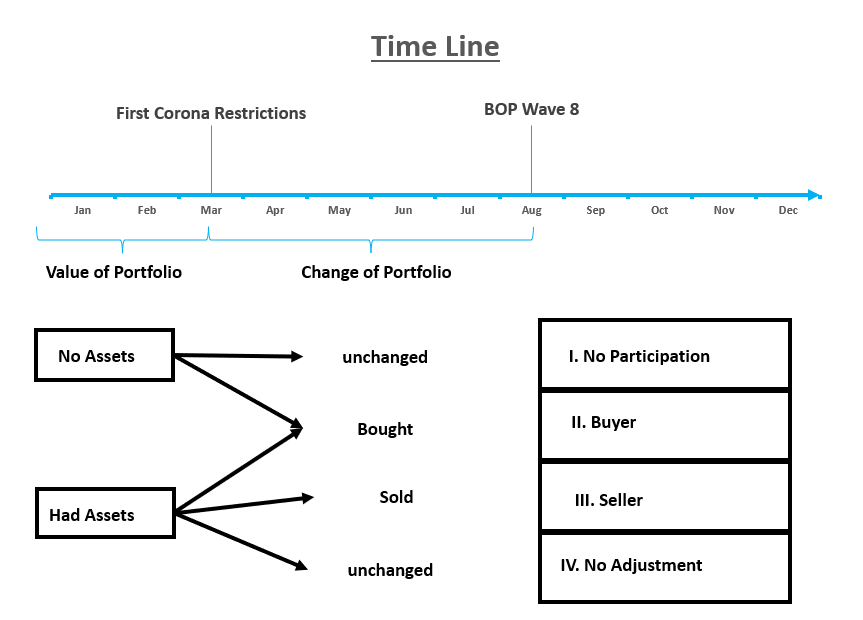
\includegraphics[width = \linewidth]{\FigDir/timeline.PNG}
	\caption{Time Line of the Questionnaire}
	\label{fig:timeline}
\end{figure}

\subsection{Expectation data}
The BOP is rich in questions regarding consumer expectations. 
\begin{enumerate}
	\item Overview of Questions
	\item My focus on Houseprices and Inflation
	\item Types of questions
	\begin{itemize}
		\item Qualitative: houseprice= mean rent and house prices; inflation = inflation...
		\item Point estimate: winsorize. 
		\item Distribution: Expected mean + SD
	\end{itemize}
\end{enumerate}

Why do I use different versions:
\textbf{\cite{potter_et_al_2017prob}: document consensus modal forecasts of federal funds rate deviate from probability-weighted means in 2016}

\textbf{\cite{diercks2021asymmetric}: extract model paths and probability-weighted means derived from the SPD dating back to 2011. Find significant skewness, blue chip lines up with modes, not probability-weighted means. Means have better forecast performance and less negative risk premia.}

$\rightarrow$: chapter 1 of handbook

\section{Results}\label{sec:results}
%This sections shows descriptive statistics of the Bundesbank Online Pilot 8th wave. %and compares it with the panel on household finances (PHF) to validate the representative nature of the data. 
Based on the questionnaire, five types can be categorized: no participation, no adjustment, bought (only), sold (only), bought and sold. Firstly, I will describe each type and alayze demographic drivers. Afterwards, I investigate the reasons for each decision. Here, I rank them and compare which factor is most important. Afterwards I conduct a principal component analysis to reduce factors and dig into heterogeneous drivers of each. Thirdly, I focus on the decision of buying and expectations. 

\subsection{Description of Types}\label{sec:des_types}
This section summarizes statistics for each type and explores the underlying factors characterizing them.

\paragraph{Who bought/sold/unchanged, and how much?}
First of all, table \ref{tab:sum_types} reports summary statistics for the different types.% -- households who never participated, who kept it unchanged but held stocks before, who bought only, sold only or bought and sold. 
The first two columns show that around half of all respondents did not hold any financial assets \textcolor{orange}{which is slightly less than in the PHF} and a quarter did have some in their portfolio prior March 2020, but did neither buy or sell any financial assets. Hence, one quarter or 497 individuals changed their portfolio between March and August 2020. \textcolor{orange}{\cite{bonaparte_et_al_2012adjustment} calculate for the US using the PSID that almost 50\% of all stock holders adjusted their portfolio within a two year span. Hence, this share has already adjusted their portfolio within 6 months. Arguably, 2020 was not a regular year and the turmoils on the stock market increased awareness to adjust the portfolio. GERMANY?! EUROPE?! COMPARISON} Interestingly, about 18 \% report, they only bought additional assets (column 3) where fonds and bonds were the most preferred asset types. Around 6 \% sold some assets, and 4.4\% bought and sold in the same time period.

\begin{table}[]
	\caption{Summary Statistics of 5 types}
	\label{tab:sum_types}
	\resizebox{\textwidth}{!}{%
		\begin{threeparttable}
			\begin{tabular}{ll|ccccccccccc}
				&  &  & \begin{tabular}[c]{@{}c@{}}no participation\\ \\ (I)\end{tabular} &  & \begin{tabular}[c]{@{}c@{}}no adjustment\\ \\ (II)\end{tabular} &  & \begin{tabular}[c]{@{}c@{}}bought\\ (only)\\ (III)\end{tabular} &  & \begin{tabular}[c]{@{}c@{}}sold\\ (only)\\ (IV)\end{tabular} &  & \begin{tabular}[c]{@{}c@{}}bought\\ and sold\\ (V)\end{tabular} &  \\ \hline
				&  &  &  &  &  &  &  &  &  &  &  &  \\
				Total & \% &  & 50.1 &  & 25.4 &  & 18.0 &  & 2.1 &  & 4.4 &  \\
				& \euro &  &  &  &  &  & 8,600 &  & -17,300 &  & 3,200 &  \\
				& sd &  &  &  &  &  & (20,900) &  & (28,600) &  & (16,900) &  \\
				&  &  &  &  &  &  &  &  &  &  &  &  \\
				Fonds & \% &  &  &  &  &  & 70.1 &  & 60.5 &  & 61.1 &  \\
				& \euro &  &  &  &  &  & 3,400 &  & -9,800 &  & 200 &  \\
				& sd &  &  &  &  &  & (10,600) &  & (17,500) &  & (5,100) &  \\
				&  &  &  &  &  &  &  &  &  &  &  &  \\
				Bonds & \% &  &  &  &  &  & 43.7 &  & 37.2 &  & 84.4 &  \\
				& \euro &  &  &  &  &  & 4,100 &  & -4,600 &  & 3,500 &  \\
				& sd &  &  &  &  &  & (12,600) &  & (16,100) &  & (16,900) &  \\
				&  &  &  &  &  &  &  &  &  &  &  &  \\
				Stocks & \% &  &  &  &  &  & 7.7 &  & 9.3 &  & 14.4 &  \\
				& \euro &  &  &  &  &  & 200 &  & -100 &  & -200 &  \\
				& sd &  &  &  &  &  & (1,600) &  & (500) &  & (2,900) &  \\
				&  &  &  &  &  &  &  &  &  &  &  &  \\
				Other & \% &  &  &  &  &  & 13.7 &  & 18.6 &  & 25.6 &  \\
				& \euro &  &  &  &  &  & 800 &  & -2,800 &  & -400 &  \\
				& sd &  &  &  &  &  & (4,900) &  & (10,800) &  & (4,900) &  \\ \hline
				&  &  &  &  &  &  &  &  &  &  &  &  \\
				n &  &  & 1,013 &  & 513 &  & 364 &  & 43 &  & 90 & \\ \hline \hline
			\end{tabular}
			\begin{tablenotes}\footnotesize
				\item[] Summary statistics of 5 types in the sample. This table shows how many of each group changed their portfolio in total and by asset type. Underneath the percentage of the population, the euro amount of the portfolio difference is reported with standard deviation in parentheses.
			\end{tablenotes}
		\end{threeparttable}
	}
\end{table}

\begin{table}[]
	\caption{Summary Statistics of 5 types (weighted)}
	\label{tab:sum_types_weighted}
	\resizebox{\textwidth}{!}{%
		\begin{threeparttable}
			\begin{tabular}{ll|ccccccccccc}
				&  &  & \begin{tabular}[c]{@{}c@{}}no participation\\ \\ (I)\end{tabular} &  & \begin{tabular}[c]{@{}c@{}}no adjustment\\ \\ (II)\end{tabular} &  & \begin{tabular}[c]{@{}c@{}}bought\\ (only)\\ (III)\end{tabular} &  & \begin{tabular}[c]{@{}c@{}}sold\\ (only)\\ (IV)\end{tabular} &  & \begin{tabular}[c]{@{}c@{}}bought\\ and sold\\ (V)\end{tabular} &  \\ \hline
				&  &  &  &  &  &  &  &  &  &  &  &  \\
				Total & \% &  & 55.1 &  & 23.0 &  & 16.1 &  & 1.9 &  & 3.9 &  \\
				& \euro &  &  &  &  &  & 6,100 &  & -11,800 &  & 1,200 &  \\
				& sd &  &  &  &  &  & (15,400) &  & (22,500) &  & (11,500) &  \\
				&  &  &  &  &  &  &  &  &  &  &  &  \\
				Fonds & \% &  &  &  &  &  & 71.9 &  & 53.4 &  & 59.2 &  \\
				& \euro &  &  &  &  &  & 2,700 &  & -5,700 &  &  0 &  \\
				& sd &  &  &  &  &  & (8,600) &  & (11,900) &  & (4,500) &  \\
				&  &  &  &  &  &  &  &  &  &  &  &  \\
				Bonds & \% &  &  &  &  &  & 44.3 &  & 41.9 &  & 81.4 &  \\
				& \euro &  &  &  &  &  & 2,400 &  & -3,300 &  & 1,700 &  \\
				& sd &  &  &  &  &  & (8,300) &  & (12,200) &  & (11,400) &  \\
				&  &  &  &  &  &  &  &  &  &  &  &  \\
				Stocks & \% &  &  &  &  &  & 7.0 &  & 12.5 &  & 13.5 &  \\
				& \euro &  &  &  &  &  & 100 &  & -100 &  & -300 &  \\
				& sd &  &  &  &  &  & (1,000) &  & (400) &  & (2,400) &  \\
				&  &  &  &  &  &  &  &  &  &  &  &  \\
				Other & \% &  &  &  &  &  & 14.3 &  & 23.6 &  & 32.1 &  \\
				& \euro &  &  &  &  &  & 900 &  & -2,700 &  & -300 &  \\
				& sd &  &  &  &  &  & (5,600) &  & (10,000) &  & (3,500) &  \\ \hline
				&  &  &  &  &  &  &  &  &  &  &  &  \\
				n &  &  & 1,013 &  & 513 &  & 364 &  & 43 &  & 90 &  \\ \hline \hline
			\end{tabular}
			\begin{tablenotes}\footnotesize
				\item[] Summary statistics of 5 types in the sample. This table shows how many of each group changed their portfolio in total and by asset type. Underneath the percentage of the population, the euro amount of the portfolio difference is reported with standard deviation in parentheses.
			\end{tablenotes}
		\end{threeparttable}
	}
\end{table}

\paragraph{Heterogeneity in who bought/sold/unchanged}
Table \ref{tab:sum_types_demo} reports a demographic breakdown for each type and confirms multiple results from the literature. Characteristics such as college degree, male, higher income and home ownership increase not only the likelihood to hold financial assets, but to trade as well. Interestingly, younger households eg the cohort below 30 years, were more likely to buy than older. \textcolor{orange}{This is in line with reports such as Flossbach and Storch... documenting an increase in stock ownership among the young.}
% + college
% - female
% + higher income
% + owner (wealth)
% + younger

%\cite{bonaparte_et_al_2012adjustment}: 'The first moment is the adjustment rate for shareholders of 46.7\% biannually...It should be noted that the 46.7\% biannual adjustment rate is not convertible into a 23.5\% annual adjustment rate, unless totally different households undertake stock adjustment in the two years. It might be, for example, that the same set of households adjust in both years, implying that the annual adjustment rate from PSID should also be 46.7\%. We take this time aggregation into account in our estimation.' \textbf{Adjustment rate}
\begin{table}[]
	\caption{Summary Statistics of 5 types}
	\label{tab:sum_types_demo}
	\resizebox{\textwidth}{!}{%
		\begin{threeparttable}
			\begin{tabular}{ll|cccccccccccc}
				&  &  & \begin{tabular}[c]{@{}c@{}}total\\ \\ (I)\end{tabular} &  & \begin{tabular}[c]{@{}c@{}}no participation\\ \\ (II)\end{tabular} &  & \begin{tabular}[c]{@{}c@{}}no adjustment\\ \\ (III)\end{tabular} &  & \begin{tabular}[c]{@{}c@{}}bought\\ (only)\\ (IV)\end{tabular} &  & \begin{tabular}[c]{@{}c@{}}sold\\ (only)\\ (V)\end{tabular} &  & \begin{tabular}[c]{@{}c@{}}bought\\ and sold\\ (VI)\end{tabular} \\ \hline
				&  &  &  &  &  &  &  &  &  &  &  &  &  \\
				\multicolumn{2}{l|}{Female} &  & 41.5 &  & 47.7 &  & 43.7 &  & 28.0 &  & 30.2 &  & 20.0 \\
				\multicolumn{2}{l|}{} &  &  &  &  &  &  &  &  &  &  &  &  \\
				\multicolumn{2}{l|}{Age} &  &  &  &  &  &  &  &  &  &  &  &  \\
				& \textless{}30 &  & 9.0 &  & 10.2 &  & 4.1 &  & 12.1 &  & 7.0 &  & 12.2 \\
				& 31-40 &  & 11.3 &  & 12.6 &  & 9.9 &  & 10.4 &  & 9.3 &  & 8.9 \\
				& 41-50 &  & 16.6 &  & 15.4 &  & 15.2 &  & 19.5 &  & 16.3 &  & 26.7 \\
				& 51-60 &  & 18.9 &  & 18.5 &  & 19.7 &  & 20.6 &  & 14.0 &  & 15.6 \\
				& 60+ &  & 41.4 &  & 40.3 &  & 48.5 &  & 35.2 &  & 46.5 &  & 35.6 \\
				&  &  &  &  &  &  &  &  &  &  &  &  &  \\
				\multicolumn{2}{l|}{HH Size} &  &  &  &  &  &  &  &  &  &  &  &  \\
				& 1 &  & 24.7 &  & 25.7 &  & 22.8 &  & 23.4 &  & 34.9 &  & 24.4 \\
				& 2 &  & 45.3 &  & 45.0 &  & 48.9 &  & 40.9 &  & 39.5 &  & 47.8 \\
				& 3 &  & 12.8 &  & 12.4 &  & 10.7 &  & 16.2 &  & 9.3 &  & 16.7 \\
				& 4 &  & 12.5 &  & 12.1 &  & 12.3 &  & 14.6 &  & 9.3 &  & 10.0 \\
				& 5+ &  & 4.6 &  & 4.5 &  & 5.1 &  & 4.7 &  & 7.0 &  & 1.1 \\
				&  &  &  &  &  &  &  &  &  &  &  &  &  \\
				\multicolumn{2}{l|}{College} &  & 29.1 &  & 24.0 &  & 32.0 &  & 35.7 &  & 37.2 &  & 38.9 \\
				&  &  &  &  &  &  &  &  &  &  &  &  &  \\
				\multicolumn{2}{l|}{Employment} &  &  &  &  &  &  &  &  &  &  &  &  \\
				& full-time &  & 42.7 &  & 38.6 &  & 38.4 &  & 55.5 &  & 51.2 &  & 56.7 \\
				& part-time &  & 11.7 &  & 13.7 &  & 11.3 &  & 8.0 &  & 4.7 &  & 8.9 \\
				& retired &  & 36.1 &  & 35.8 &  & 42.3 &  & 29.7 &  & 32.6 &  & 31.1 \\
				& unemployed &  & 9.6 &  & 11.8 &  & 8.0 &  & 6.9 &  & 11.6 &  & 3.3 \\
				&  &  &  &  &  &  &  &  &  &  &  &  &  \\
				\multicolumn{2}{l|}{HH income} &  &  &  &  &  &  &  &  &  &  &  &  \\
				& \textless{}1500 &  & 12.2 &  & 16.4 &  & 9.9 &  & 4.7 &  & 11.6 &  & 8.9 \\
				& 1500-3000 &  & 31.9 &  & 34.8 &  & 31.2 &  & 27.7 &  & 20.9 &  & 25.6 \\
				& 3000-5000 &  & 37.2 &  & 35.1 &  & 39.2 &  & 42.3 &  & 34.9 &  & 30.0 \\
				& 5000-8000 &  & 16.0 &  & 12.1 &  & 17.0 &  & 21.2 &  & 32.6 &  & 24.4 \\
				& 8000+ &  & 2.7 &  & 1.5 &  & 2.7 &  & 4.1 &  & 0.0 &  & 11.1 \\
				&  &  &  &  &  &  &  &  &  &  &  &  &  \\
				\multicolumn{2}{l|}{Owner} &  & 62.4 &  & 54.0 &  & 71.7 &  & 73.6 &  & 60.5 &  & 60.0 \\ 
				& &  &  &  &  &  &  &  &  &  &  &  &  \\ \hline \hline
			\end{tabular}
			\begin{tablenotes}\footnotesize
				\item[] Summary statistics of the demographics of the total sample and the 5 types. This table shows the percentage of respondents in each type.
			\end{tablenotes}
		\end{threeparttable}
	}
\end{table}

\subsection{Reasons of behavior}
In the previous section, we have seen that around 1,500 individuals did adjust their financial asset holdings, while a quarter of all observations bought and/or sold some assets. This section investigates the underlying reasons of the respective behavior.

\subsubsection{Reasons No Participation}
First, I will focus on the question: \textit{what prevents individuals from holding stocks?}\footnote{The question reads: 'Why did you decide not to buy any asset(s) during the coronavirus pandemic?'} 

Table \ref{tab:reason_nostocks} reports the answers of individuals who did not hold any financial assets prior March 2020 and decided not to buy any afterwards. Individuals could rate each reason from 1 'strongly disagree' to 4 'strongly agree'. The first column reports the share of individuals who rated the reason 'fully agree', while the second column adds respondents who also 'rather agree''d. The third column shows the mean and the fourth column reports the mean of the standardized variable. The latter was constructed similar to \cite{choi_2020}, where each answer is standardized using the average reported answer of all reasons per person and its standard deviation. The advantage is that each reason becomes more comparable as the standardisation takes care of the fact that the perception of 'agreement' might differ among participants. Additionally, observations where all answers receive the same score are filtered out.

%average reported answer per person is subtracted from the answer for each reason and divided by the standard error 
While there is not one or two dominant reasons, a conglomeration of factors seem to be important. The two most important factors which are supported by around 70\% of respondents and almost half say they fully agree are \textit{lack of information} and \textit{no interest}, followed by distrust in the stock market, time constraints and peer-effects (around 60\% agree). Interestingly, \textit{no savings} plays still for more than 50\% a larger role, but ranks relatively low. In contrast to \cite{choi_2020}, where 'Wealth too small to invest in stocks' is the most important reason which is interpreted as 'participation costs'. By rephrasing it and asking about savings which could be invested in all sort of asset classes, a lack of such seems to to be less important.

Looking at the lower end of the scale, the shock of the stock market break due to covid-19, which would be in line with \cite{malmendier_2011} is still for almost a quarter important, but seems not to play a predominant role. Similarly, costs such as bank fees and transaction costs and moral issues are only important for a small fraction of households.

\begin{table}[]
	\caption{Summary Statistics: Reasons No Participation}
	\label{tab:reason_nostocks}
	\resizebox{\textwidth}{!}{%
		\begin{threeparttable}
			\begin{tabular}{l|lccccccc}
				&  & \begin{tabular}[c]{@{}c@{}}Fully agree\\ (I)\end{tabular} &  & \begin{tabular}[c]{@{}c@{}}At least\\ rather agree\\ (II)\end{tabular} &  & \begin{tabular}[c]{@{}c@{}}Mean\\ (III)\end{tabular} &  & \begin{tabular}[c]{@{}c@{}}Standardized\\ (III)\end{tabular} \\ \hline
				&  &  &  &  &  &  &  &  \\
				information &  & 50.52\% &  & 72.80\% &  & 3.25 &  & 0.58 \\
				no interest &  & 47.49\% &  & 69.88\% &  & 3.17 &  & 0.47 \\
				distrust &  & 37.99\% &  & 63.03\% &  & 3.00 &  & 0.27 \\
				too risky &  & 34.77\% &  & 59.35\% &  & 2.88 &  & 0.17 \\
				no time &  & 33.37\% &  & 57.89\% &  & 2.83 &  & 0.09 \\
				peer-effect &  & 30.22\% &  & 51.31\% &  & 2.70 &  & -0.08 \\
				no savings &  & 30.32\% &  & 53.92\% &  & 2.73 &  & -0.12 \\
				high   valuations &  & 17.52\% &  & 51.77\% &  & 2.61 &  & -0.15 \\
				shock &  & 23.91\% &  & 46.28\% &  & 2.53 &  & -0.22 \\
				costs &  & 19.95\% &  & 42.88\% &  & 2.44 &  & -0.34 \\
				moral &  & 16.27\% &  & 32.39\% &  & 2.17 &  & -0.70\\ 
				&  &  &  &  &  &  &  &  \\\hline \hline
			\end{tabular}
			\begin{tablenotes}\footnotesize
				\item[] Summary statistics of reasons why households did not adjust their portfolio between March and August 2020. The first column reports the share of individuals who rated the reason 'fully agree', while the second column doe it for 'fully agree or 'rather agree'. The third column shows the mean (1-4 with 4 'fully agree') and the fourth column reports the mean of the standardized variable.
			\end{tablenotes}
		\end{threeparttable}
	}
\end{table}

% \textcolor{orange}{table regression nostocks and demographics \label{tab:reg_nostocks_dem}}

% Table \ref{tab:reg_nostocks_dem} shows the six most important reasons by demographics to analyse heterogeneity across them. Here, the standardized reported answers are regressed on household demographics. A large variation within reasons is captured by cohort effects. For instance, the \textit{lack of information} (column I) is more prominent for younger households which is true for \textit{time} constraints (column V), as well. Contrarily, \textit{distrust} in the sock market (column III) increases with age. Apart from that, we find an indication that \textit{lack of information} is less important for high income households and female respondents seem to be less interested (column II).
% lack of information more important for younger households not important for high income households.
% distrust increases with age
% no time important for younger households
% female less interest

% \textcolor{orange}{compare with literature!}

\paragraph{Principal Component Analysis}

Next, I conduct a principal component analysis to show how many factors are relevant and how they relate to each other. Table \ref{tab:pca_reason_nopart} shows the result following \cite{choi_2020, tabachnick_fidell_2007} and considering components with an eigenvalue of more than 1 as well as focusing on variables with a loading factor of more than 0.32.\footnote{The results do not change if rotated factors are used.}

Three factors explain 47.45\% of the variance in the data. The first factor captures \textit{risk aversion} of households. It consists of four variables: 'Financial assets are too risky for me at the moment', 'I do not trust the stock market', 'The recent collapse in financial market prices puts me off', and 'Prices will fall again or fall lower'. 

The second factor captures \textit{lack of resources}. It consists of 'lack of interest', 'lack of information', 'lack of time', and 'lack of savings'. While the first component is about risk preferences which are not easy to change, this factor opens up the opportunity to increase stock holdings by focusing on these variables.

The third factor consists of 'lack of savings' and 'moral issues', while the latter is negatively correlated. Hence, these households would like to invest, but the lack of additional money prevents them from doing it.

\begin{table}[]
	\caption{Principal Component Analysis: Reasons No Participation}
	\label{tab:pca_reason_nopart}
	\resizebox{\textwidth}{!}{%
		\begin{threeparttable}
			\begin{tabular}{lcclcclc}
				\hline
				\multicolumn{2}{c}{\begin{tabular}[c]{@{}c@{}}Comp   1\\ risk aversion\end{tabular}} &  & \multicolumn{2}{c}{\begin{tabular}[c]{@{}c@{}}Comp   2\\ lack of resources\end{tabular}} &  & \multicolumn{2}{c}{\begin{tabular}[c]{@{}c@{}}Comp   3\\ no savings\end{tabular}} \\ \cline{1-2} \cline{4-5} \cline{7-8} 
				&  &  &  &  &  &  &  \\
				too risky & 0.42 &  & no interest & 0.47 &  & no savings & 0.64 \\
				distrust & 0.42 &  & information & 0.40 &  & moral & -0.60 \\
				shock & 0.37 &  & no time & 0.40 &  &  &  \\
				high valuations & 0.35 &  & no savings & 0.34 &  &  &  \\
				&  &  & shock & -0.33 &  &  &  \\
				&  &  &  &  &  &  &  \\ \hline \hline
			\end{tabular}
			\begin{tablenotes}\footnotesize
				\item[] Caption
			\end{tablenotes}
		\end{threeparttable}
	}
\end{table}

In another step, a regression analysis evaluates driving factors of each component. For this, the mean value of all standardized variable is used to calculate the average value for each component. The resulting indicator is then regressed on demographics.

Table \ref{tab:reg_nopart_dem} shows that the first component or \textit{risk aversion} increases with age, while the second one (\textit{lack of resources}) has the opposite dynamic. Lastly, \textit{no savings} depends on the work status and income level. 

\textcolor{orange}{Summary \& Interpretation: A result of this exercise is that many factors play an important role and can predict or explain why people do not participate in financial markets. Nevertheless, these reasons can be grouped into three big components which are driven by either a lifecycle pattern or by income levels. Hence, if someone wants to model stock market behavior, these mechanisms can be easily implemented.}

\begin{table}[] \centering
	\def\sym#1{\ifmmode^{#1}\else\(^{#1}\)\fi}
	\caption{Regression Table: Reason No Participation and Demographics \label{tab:reg_nopart_dem}}
	\resizebox{0.5\textwidth}{!}{%
		\begin{threeparttable}
			\begin{tabular}{l*{3}c}
				\hline\hline
				                    &\multicolumn{1}{c}{(1)}&\multicolumn{1}{c}{(2)}&\multicolumn{1}{c}{(3)}\\
                    &\multicolumn{1}{c}{\shortstack{Risk \\ Aversion}}&\multicolumn{1}{c}{\shortstack{Lack of \\ Resources}}&\multicolumn{1}{c}{\shortstack{No\\ Savings}}\\
\hline
1500-3000           &      -0.005         &      -0.010         &      -0.100\sym{**} \\
                    &     (0.048)         &     (0.047)         &     (0.045)         \\
[1em]
3000-5000           &       0.006         &      -0.044         &      -0.161\sym{***}\\
                    &     (0.049)         &     (0.045)         &     (0.045)         \\
[1em]
5000-8000           &      -0.028         &      -0.095         &      -0.263\sym{***}\\
                    &     (0.063)         &     (0.060)         &     (0.053)         \\
[1em]
8000+               &       0.014         &      -0.086         &      -0.191\sym{***}\\
                    &     (0.087)         &     (0.068)         &     (0.072)         \\
[1em]
31-40               &       0.078         &      -0.050         &      -0.055         \\
                    &     (0.058)         &     (0.062)         &     (0.050)         \\
[1em]
41-50               &       0.091         &      -0.073         &      -0.008         \\
                    &     (0.059)         &     (0.064)         &     (0.051)         \\
[1em]
51-60               &       0.167\sym{***}&      -0.078         &      -0.003         \\
                    &     (0.060)         &     (0.062)         &     (0.050)         \\
[1em]
60+                 &       0.191\sym{***}&      -0.153\sym{**} &      -0.009         \\
                    &     (0.071)         &     (0.074)         &     (0.058)         \\
\hline
Observations        &         906         &         926         &         917         \\
Adjusted \(R^{2}\)  &       0.061         &       0.023         &       0.053         \\
Controls            &         Yes         &         Yes         &         Yes         \\

				\hline\hline
			\end{tabular}
			\begin{tablenotes}\footnotesize
				\item[] Standard errors in parentheses. \sym{*} \(p<0.10\), \sym{**} \(p<0.05\), \sym{***} \(p<0.01\)
				\item[] Additional controls are college, labor status, gender, children, home ownership
				\item[] Data source: BOP Wave 8
			\end{tablenotes}
		\end{threeparttable}
	}
\end{table}


\subsubsection{Reasons No Adjustment}
Next, I focus on individuals who held some financial assets, but did not buy or sell between March and August. These reasons refer more to 'adjustment costs', meaning the 'participation costs' are already paid, but these factors prevent them from investing \textit{more}. Or rephrasing it, the question is \textit{Why don't households adjust their portfolio?}

\begin{table}[]
	\caption{Summary Statistics: Reasons No Adjustment}
	\label{tab:reason_unchanged}
	\resizebox{\textwidth}{!}{%
		\begin{threeparttable}
			\begin{tabular}{l|lccccccc}
				&  & \begin{tabular}[c]{@{}c@{}}Fully agree\\ (I)\end{tabular} &  & \begin{tabular}[c]{@{}c@{}}At least\\ rather agree\\ (II)\end{tabular} &  & \begin{tabular}[c]{@{}c@{}}Mean\\ (III)\end{tabular} &  & \begin{tabular}[c]{@{}c@{}}Standardized\\ (III)\end{tabular} \\ \hline
				&  &  &  &  &  &  &  &  \\
				too risky &  & 20.47\% &  & 55.52\% &  & 2.53 &  & 0.31 \\
				high   valuations &  & 9.47\% &  & 48.62\% &  & 2.39 &  & 0.09 \\
				no time &  & 17.05\% &  & 49.39\% &  & 2.38 &  & 0.11 \\
				no savings &  & 18.25\% &  & 42.20\% &  & 2.30 &  & -0.06 \\
				peer-effect &  & 17.24\% &  & 36.07\% &  & 2.12 &  & -0.19 \\
				costs &  & 10.67\% &  & 32.40\% &  & 2.09 &  & -0.28 \\ 
				&  &  &  &  &  &  &  &  \\\hline \hline
			\end{tabular}
			\begin{tablenotes}\footnotesize
				\item[] Summary statistics of reasons why households did not adjust their portfolio between March and August 2020, but held stocks before. The first column reports the share of individuals who rated the reason 'fully agree', while the second column doe it for 'fully agree or 'rather agree'. The third column shows the mean (1-4 with 4 'fully agree') and the fourth column reports the mean of the standardized variable.
			\end{tablenotes}
		\end{threeparttable}
	}
\end{table}

Table \ref{tab:reason_unchanged} reports the results. As a general note, the reasons in question did not score as high compared to the table above, where the most important reason had a mean of 3.25 compared to 2.53 here. \textcolor{orange}{Hence, while a large literature focuses on participation constraints, the question which reasons prevent individuals from holding larger shares in financial assets might need further attention. Are these the same or other factors which lead to non-participation?}

What can be seen is that uncertainty and the risk of a downturn of the stock market prevented households to buy or sell any of their assets. \textcolor{orange}{These points seem understandable as volatility increased in the market due to covid and the stock market increased heavily between March and August. As even economists could only guess whether the economy would have a L,V,W or K shaped recovery, how should households know?}

Interestingly, time constraints are similarly important. While \textcolor{orange}{\cite{choi_2020} argue that only 3\% of his sample report that time issues play a role over a long period (he asks for participation over all without specifying a time period), choosing the 6 month span shows that household do argue that time constraints are important. Of course, this could be due to living in a pandemic, where home office and schooling puts an additional burden on households. Contrarily, households could also have more time on their hand due to restrictions on activities with friends (eating in a restaurant, meeting in a bar or going on vacations).}
%Interestingly, \textit{time} constraints play an important reason as well. This factor is quite disperse as lockdown measurements could either increase time (less time for activities with friends/ commuting to work...), some households had an additional burden with homeschooling and he like. Hence, it is not surprising that households with children thought time constraints are more important than households without children. \textcolor{orange}{not captured in regression output!}

%\textcolor{orange}{table regression unchanged and demographics. Maybe add small children?!}\label{tab:reg_unchanged_dem}

%Table \ref{tab:reg_unchanged_dem} reports heterogeneity across households which is for \textit{no additional savings} (column 4) and \textit{peer-effect} (column 5) captured by a lifecycle pattern. For the former, saving constraints are more important for older households. \textcolor{orange}{This seems to be counter intuitive at first, as income increases with age. However, older households might already have different saving arrangements in place such as retirement schemes which does not give room for additional purchases.} Additionally, the peer effect seems to be stronger for younger households. 

%\textcolor{orange}{discussion?!}
% no additional savings more important for older households while peer effects are more prominent for younger households

\paragraph{Principal Component Analysis}
By conducting a PCA, two factors explain 60.20\% of the variation. They divide the reasons why people did not adjust their portfolio in two groups. The first captures \textit{bad timing}. It consists of 'high valuation', 'too risky', 'costs', and 'peer-effects'. All of them indicate that the person is aware of the stock market, but did not change the portfolio as the timing of investment is bad. Either because the market is too volatile or because costs or peer-effects prevent them.

The second factor captures \textit{lack of time} and consists of 'lack of savings' (negative), 'lack of peers' and 'lack of time'. Here, the household might be willing to buy, but restricted resources prevent them.

\textcolor{orange}{Summary and Interpretation: Based on the findings, households waited to invest further either because they thought the timing is bad, or other obligations prevented them from allocating time into investment decisions.}

\begin{table}[]
	\caption{ Principal Component Analysis: No Adjustment}
	\label{tab:reason_unchanged}
	\resizebox{\textwidth}{!}{%
		\begin{threeparttable}
			\begin{tabular}{llcll}
				\hline
				\multicolumn{2}{c}{\begin{tabular}[c]{@{}c@{}}Comp   1\\ bad timing\end{tabular}} &  & \multicolumn{2}{c}{\begin{tabular}[c]{@{}c@{}}Comp   2\\ lack of time\end{tabular}} \\ \cline{1-2} \cline{4-5} 
				& \multicolumn{1}{c}{} &  &  & \multicolumn{1}{c}{} \\
				too risky & 0.63 &  & no savings & -0.70 \\
				high valuations & 0.58 &  & peer effect & 0.55 \\
				costs & 0.49 &  & no time & 0.45 \\
				&  &  &  &  \\  \hline \hline
			\end{tabular}
			\begin{tablenotes}\footnotesize
				\item[] Notes
			\end{tablenotes}
		\end{threeparttable}
	}
\end{table}

\subsubsection{Reasons bought}
The first two paragraphs focused on what prevents households from holding any stocks or only to a limited amount. Now, we ask the question \textit{What factors encourage households to purchase financial assets?}

\begin{table}[]
	\caption{Summary Statistics: Reasons Bought}
	\label{tab:reason_bought}
	\resizebox{\textwidth}{!}{%
		\begin{threeparttable}
			\begin{tabular}{l|lccccccc}
				&  & \begin{tabular}[c]{@{}c@{}}Fully agree\\ (I)\end{tabular} &  & \begin{tabular}[c]{@{}c@{}}At least\\ rather agree\\ (II)\end{tabular} &  & \begin{tabular}[c]{@{}c@{}}Mean\\ (III)\end{tabular} &  & \begin{tabular}[c]{@{}c@{}}Standardized\\ (III)\end{tabular} \\ \hline
				&  &  &  &  &  &  &  &  \\
				low valuations &  & 38.74\% &  & 64.08\% &  & 2.79 &  & 0.90 \\
				plan &  & 43.54\% &  & 62.07\% &  & 2.76 &  & 0.92 \\
				time &  & 8.09\% &  & 26.59\% &  & 1.77 &  & -0.07 \\
				information &  & 7.60\% &  & 24.22\% &  & 1.70 &  & -0.15 \\
				less   consumption &  & 3.88\% &  & 18.73\% &  & 1.58 &  & -0.29 \\
				more income &  & 4.33\% &  & 19.88\% &  & 1.57 &  & -0.31 \\
				peer-effect &  & 4.15\% &  & 13.87\% &  & 1.49 &  & -0.36 \\
				bank fees &  & 0.38\% &  & 3.52\% &  & 1.21 &  & -0.65 \\ 
				&  &  &  &  &  &  &  &  \\\hline \hline
			\end{tabular}
			\begin{tablenotes}\footnotesize
				\item[] Summary statistics of reasons why households bought financial assets between March and August 2020. The first column reports the share of individuals who rated the reason 'fully agree', while the second column doe it for 'fully agree or 'rather agree'. The third column shows the mean (1-4 with 4 'fully agree') and the fourth column reports the mean of the standardized variable.
			\end{tablenotes}
		\end{threeparttable}
	}
\end{table}

Table \ref{tab:reason_bought} reports the answers to the question \textit{'Why did you decide to buy the asset(s) after the coronavirus pandemic began?'} The picture is much clearer in this case, as more than 60\% at least rather agreed and around 40\% fully agreed with two statements. First, \textit{low valuation}, meaning expecting higher stock market values in the future led to their investment decision, and second, households bought assets using a (pre-existing) \textit{savings plan}. \textcolor{orange}{These insights can be easily implemented in economic models where a share of households save using savings plan with a fixed amount invested each period and households who actively take advantage of low valuations.} 

Looking at the lower end, additional time and information played for around a quarter of respondents an important role. \textcolor{orange}{These would be factors, policy makers could focus on increasing stock market participation rates.} An increase in savings due either less consumption or more income led around 20\% to a purchase of additional assets. Finally, peer-effects which have been focused on by many scholars, seems to be a rather less important factor for the average buyer and bank fees -- eg actual costs of transaction -- have a very small elasticity.

%\textcolor{orange}{table regression bought and demographics with FT buyer and has bought and sold}
\begin{table}[]
	\def\sym#1{\ifmmode^{#1}\else\(^{#1}\)\fi}
	\caption{Regression Table: Reason bought and Demographics \label{tab:reg_bought_dem}}
	\resizebox{\textwidth}{!}{%
		\begin{threeparttable}
			\begin{tabular}{l*{7}{c}}
				\hline\hline
				 &\multicolumn{1}{c}{(1)}&\multicolumn{1}{c}{(2)}&\multicolumn{1}{c}{(3)}&\multicolumn{1}{c}{(4)}&\multicolumn{1}{c}{(5)}&\multicolumn{1}{c}{(6)}&\multicolumn{1}{c}{(7)}\\
                    &\multicolumn{1}{c}{\shortstack{low \\ valuation}}&\multicolumn{1}{c}{\shortstack{savings \\ plan}}&\multicolumn{1}{c}{\shortstack{more\\ time}}&\multicolumn{1}{c}{\shortstack{more\\ information}}&\multicolumn{1}{c}{\shortstack{less\\ consumption}}&\multicolumn{1}{c}{\shortstack{more\\ income}}&\multicolumn{1}{c}{\shortstack{peer \\effect}}\\
\hline
college             &      -0.070         &       0.104         &      -0.162         &      -0.052         &       0.035         &      -0.054         &       0.200\sym{**} \\
                    &     (0.123)         &     (0.152)         &     (0.103)         &     (0.112)         &     (0.085)         &     (0.087)         &     (0.090)         \\
[1em]
1500-3000           &      -0.802\sym{**} &       0.693\sym{*}  &       0.094         &      -0.076         &       0.497\sym{***}&       0.174         &      -0.582\sym{*}  \\
                    &     (0.316)         &     (0.377)         &     (0.266)         &     (0.375)         &     (0.159)         &     (0.282)         &     (0.340)         \\
[1em]
3000-5000           &      -0.593\sym{*}  &       0.912\sym{**} &       0.139         &      -0.132         &       0.328\sym{**} &      -0.087         &      -0.513         \\
                    &     (0.330)         &     (0.404)         &     (0.270)         &     (0.374)         &     (0.147)         &     (0.270)         &     (0.338)         \\
[1em]
5000-8000           &      -0.237         &       0.510         &       0.145         &      -0.237         &       0.350\sym{**} &       0.089         &      -0.516         \\
                    &     (0.330)         &     (0.407)         &     (0.285)         &     (0.373)         &     (0.171)         &     (0.276)         &     (0.338)         \\
[1em]
8000+               &      -0.243         &       0.314         &      -0.133         &      -0.338         &       0.359\sym{*}  &       0.108         &       0.132         \\
                    &     (0.359)         &     (0.433)         &     (0.285)         &     (0.419)         &     (0.205)         &     (0.306)         &     (0.368)         \\
[1em]
31-40               &      -0.192         &       0.315         &      -0.520\sym{***}&       0.154         &       0.001         &       0.263         &      -0.279\sym{*}  \\
                    &     (0.216)         &     (0.253)         &     (0.170)         &     (0.239)         &     (0.167)         &     (0.177)         &     (0.148)         \\
[1em]
41-50               &      -0.250         &       0.646\sym{**} &      -0.379\sym{*}  &      -0.142         &       0.006         &       0.117         &      -0.415\sym{***}\\
                    &     (0.169)         &     (0.252)         &     (0.194)         &     (0.181)         &     (0.137)         &     (0.145)         &     (0.137)         \\
[1em]
51-60               &      -0.551\sym{***}&       0.476\sym{*}  &      -0.289         &       0.138         &      -0.026         &       0.157         &      -0.358\sym{***}\\
                    &     (0.195)         &     (0.273)         &     (0.206)         &     (0.210)         &     (0.140)         &     (0.157)         &     (0.138)         \\
[1em]
60+                 &      -0.510\sym{*}  &       0.542\sym{*}  &      -0.256         &       0.430\sym{*}  &      -0.233         &      -0.053         &      -0.390\sym{**} \\
                    &     (0.269)         &     (0.288)         &     (0.239)         &     (0.228)         &     (0.188)         &     (0.155)         &     (0.172)         \\
[1em]
first time          &       0.181         &      -0.871\sym{***}&       0.703\sym{***}&       0.043         &      -0.256\sym{**} &       0.370         &      -0.069         \\
                    &     (0.198)         &     (0.268)         &     (0.186)         &     (0.236)         &     (0.103)         &     (0.225)         &     (0.250)         \\
[1em]
bought \& sold      &       0.510\sym{***}&      -0.961\sym{***}&       0.216\sym{*}  &       0.454\sym{***}&      -0.165\sym{*}  &      -0.024         &       0.035         \\
                    &     (0.132)         &     (0.172)         &     (0.130)         &     (0.171)         &     (0.093)         &     (0.095)         &     (0.099)         \\
\hline
Observations        &         426         &         429         &         429         &         428         &         429         &         429         &         425         \\
Adjusted \(R^{2}\)  &       0.099         &       0.193         &       0.139         &       0.056         &       0.054         &       0.034         &       0.170         \\
Controls            &         Yes         &         Yes         &         Yes         &         Yes         &         Yes         &         Yes         &         Yes         \\
				\hline\hline
			\end{tabular}
			\begin{tablenotes}\footnotesize
				\item[] Standard errors in parentheses
				\item[] Dependent variable: Reason bought (standardized).
				\item[] Additional controls are labor status, gender, children, home ownership
				\item[] Data source: BOP Wave 8
				\item[] \sym{*} \(p<0.10\), \sym{**} \(p<0.05\), \sym{***} \(p<0.01\)
			\end{tablenotes}
		\end{threeparttable}
	}
\end{table}

By focusing on household heterogeneity in table \ref{tab:reg_bought_dem}, we add a dummy for first time buyers and if the individual bought and sold as well to capture re-balancing effects. Additionally, the regression controls for labor status, gender, if the respondent has children living in the household and home ownership status. As they do not add any value, it is suppressed in the table.

Most variation can be captured by either an income or cohort effect. Column 1 shows that \textit{low valuation} is more important for respondents with less than 1500 Euro monthly income, while having a \textit{savings plan} or more savings due to \textit{less consumption} has the opposite effect. For the cohort effect, the reasons \textit{more time} and \textit{peer effect} are more prominent for people below 30.

Interestingly, looking at first time buyers, having \textit{more time} (column 3) is very important. \textcolor{orange}{This could explain the increase in stock holdings in Germany. Young households, who had more time on their hand started to invest.}

Lastly, households who rebalanced did so because of the \textit{low valuation}, and additional \textit{time} and \textit{information}. These households are less likely to are guided by \textit{savings plans}.

% The results can be categorized in four groups, first a cohort effect is visible for \textit{low valuation} column (I). This reason seems to be less important for older households, but more important for retired \textcolor{orange}{?!}. Second, a wealth effect can be seen in column II, where a \textit{savings plan} is most important for middle income households (1,500-5,000\euro) and the reason that \textit{more income} led to a purchase is larger for households with less than 1,500\euro, as well as college graduates.

% Third, while most of these households already hold some financial assets before purchasing more, we capture the behavior of 24 first time buyers as well. While this is a very limited amount of households, we still find that a \textit{savings plan} is less important for their choice -- which seems obvious --, and, more importantly, the additional \textit{time} (column 3) plays a large significant effect.  \textcolor{orange}{Discussion: Hence, covid restrictions could have led to an increase in stock market participation rates which could have permanent effects.... Peer effect positive only 10\% significance level}

% \textcolor{orange}{First time and college: + low valuation/ + more income}

% Lastly, households who bought and sold where more likely to report higher values for \textit{low valuation} and \textit{additional information} in comparison to households who only bought. Conversely, households who bought only where more likely to state the reason \textit{savings plan}. \textcolor{orange}{savingsplan: less reshuffeling themselves? If rebalanced: due to valuation and additional information... Time positive at 10\% level: needs time to rebalance. Invest in what?}
% cohort, wealth, first time buyers:
% cohort: low valuation less important for older households; but more for retired!
% wealth: more income: more important for households with less than 1500 income and college graduates; plan: middle income more important (1.500-5.000)
% first time: savings plan is less important (duh), time is more important!, 
\paragraph{Principal Component Analysis}

\begin{table}[]
	\caption{ Principal Component Analysis: Has Bought}
	\label{tab:PCA_reason_bough}
	\resizebox{\textwidth}{!}{%
		\begin{threeparttable}
			\begin{tabular}{llclcclc}
				\hline
				\multicolumn{2}{c}{\begin{tabular}[c]{@{}c@{}}Comp   1\\ additional resources\end{tabular}} &  & \multicolumn{2}{c}{\begin{tabular}[c]{@{}c@{}}Comp   2\\ active vs passive\end{tabular}} &  & \multicolumn{2}{c}{\begin{tabular}[c]{@{}c@{}}Comp   3\\ TBD?\end{tabular}} \\ \cline{1-2} \cline{4-5} \cline{7-8} 
				& \multicolumn{1}{c}{} &  &  &  &  &  &  \\
				costs & 0.57 &  & plan & \multicolumn{1}{l}{-0.69} &  & less consumption & \multicolumn{1}{l}{0.70} \\
				more income & 0.51 &  & low valuations & \multicolumn{1}{l}{0.58} &  & peer effect & \multicolumn{1}{l}{0.67} \\
				information & 0.49 &  &  &  &  &  &  \\
				time & 0.37 &  &  &  &  &  &  \\
				& \multicolumn{1}{c}{} &  &  &  &  &  &  \\ \hline
			\end{tabular}
			\begin{tablenotes}\footnotesize
				\item[] Notes
			\end{tablenotes}
		\end{threeparttable}
	}
\end{table}


\paragraph{Active vs Passive Buyers}
Interestingly, the two reasons with the highest scores are part of the same component with opposite sign. Hence, respondents were either active or passive buyers. To dig deeper, I group everyone who reported a \textit{savings plan} was an above average reason as \textit{passive buyer}, while grouping everyone who does the same with \textit{low valuation} and is not a passive buyer, as \textit{active}.

Passive buyers: 287 $\rightarrow$ 64\%
Active buyers: 137 $\rightarrow$ 30 \%
Neither: 30 $\rightarrow$ 6\%

Next, I use a probit model to see which demographic characteristics determine active or passive buyers, as well as the other reasons for buying. Table \ref{tab:reg_bought_active_passive} shows the results. The first two columns contain the full sample, while the others condition on having bought. This exercise shows that younger (below 30), wealthier (home owner) households are more likely to be active buyers. Additionally, they are more likely to be first time buyers or people who rebalanced during the 6 month period.

Columns 5 and 6 show that active buyers were also more likely to state that additional time, information, income and a peer-effect led them to the decision to buy. Contrarily, passive buyers are less responsive to these factors.

\begin{table}[]
	\def\sym#1{\ifmmode^{#1}\else\(^{#1}\)\fi}
	\caption{Regression Table: Active vs Passive buyers (Probit) \label{tab:reg_bought_active_passive}}
	\resizebox{\textwidth}{!}{%
		\begin{threeparttable}
			\begin{tabular}{l*{7}{c}}
				\hline\hline
				\begin{table}[ht!]
	\centering
	\def\sym#1{\ifmmode^{#1}\else\(^{#1}\)\fi}
	\caption{Regression Table: Active vs Passive buyers (Probit) \label{tab:reg_bought_active_passive}}
	\resizebox{\textwidth}{!}{%
		\begin{threeparttable}
			\begin{tabular}{l*{15}{c}}
				\hline\hline
				                    &            &\multicolumn{1}{c}{(1)}&            &\multicolumn{1}{c}{(2)}&            &\multicolumn{1}{c}{(3)}&            &\multicolumn{1}{c}{(4)}&            &\multicolumn{1}{c}{(5)}&            &\multicolumn{1}{c}{(6)}\\
                    &            &\multicolumn{1}{c}{\shortstack{active}}&            &\multicolumn{1}{c}{\shortstack{passive}}&            &\multicolumn{1}{c}{\shortstack{active}}&            &\multicolumn{1}{c}{\shortstack{passive}}&            &\multicolumn{1}{c}{\shortstack{active}}&            &\multicolumn{1}{c}{\shortstack{passive}}\\
\hline
                    &            &                     &            &                     &            &                     &            &                     &            &                     &            &                     \\
owner               &            &       0.492\sym{***}&            &       0.106         &            &       0.552\sym{***}&            &      -0.395\sym{**} &            &       0.535\sym{***}&            &      -0.485\sym{**} \\
                    &            &     (0.130)         &            &     (0.100)         &            &     (0.198)         &            &     (0.192)         &            &     (0.200)         &            &     (0.203)         \\
[1em]
$<30$               &            &       0.520\sym{***}&            &       0.131         &            &       0.612\sym{**} &            &      -0.262         &            &       0.416         &            &      -0.215         \\
                    &            &     (0.169)         &            &     (0.139)         &            &     (0.246)         &            &     (0.252)         &            &     (0.256)         &            &     (0.274)         \\
[1em]
first time          &            &       1.715\sym{***}&            &       0.710\sym{**} &            &       0.715\sym{**} &            &      -0.939\sym{***}&            &       0.424         &            &      -0.591\sym{*}  \\
                    &            &     (0.342)         &            &     (0.342)         &            &     (0.344)         &            &     (0.341)         &            &     (0.330)         &            &     (0.324)         \\
[1em]
bought \& sold      &            &       1.636\sym{***}&            &       0.883\sym{***}&            &       0.653\sym{***}&            &      -0.806\sym{***}&            &       0.767\sym{***}&            &      -0.948\sym{***}\\
                    &            &     (0.201)         &            &     (0.185)         &            &     (0.215)         &            &     (0.212)         &            &     (0.225)         &            &     (0.223)         \\
[1em]
time                &            &                     &            &                     &            &                     &            &                     &            &       0.703\sym{***}&            &      -1.152\sym{***}\\
                    &            &                     &            &                     &            &                     &            &                     &            &     (0.126)         &            &     (0.136)         \\
[1em]
information         &            &                     &            &                     &            &                     &            &                     &            &       0.206\sym{*}  &            &      -0.899\sym{***}\\
                    &            &                     &            &                     &            &                     &            &                     &            &     (0.121)         &            &     (0.128)         \\
[1em]
less consumption    &            &                     &            &                     &            &                     &            &                     &            &       0.224         &            &      -0.820\sym{***}\\
                    &            &                     &            &                     &            &                     &            &                     &            &     (0.170)         &            &     (0.167)         \\
[1em]
more income         &            &                     &            &                     &            &                     &            &                     &            &       0.415\sym{**} &            &      -1.120\sym{***}\\
                    &            &                     &            &                     &            &                     &            &                     &            &     (0.172)         &            &     (0.157)         \\
[1em]
costs               &            &                     &            &                     &            &                     &            &                     &            &       0.871\sym{***}&            &      -2.069\sym{***}\\
                    &            &                     &            &                     &            &                     &            &                     &            &     (0.270)         &            &     (0.301)         \\
[1em]
peer effect         &            &                     &            &                     &            &                     &            &                     &            &       0.742\sym{***}&            &      -1.534\sym{***}\\
                    &            &                     &            &                     &            &                     &            &                     &            &     (0.166)         &            &     (0.170)         \\
\hline
Observations        &            &        2018         &            &        2018         &            &         454         &            &         454         &            &         431         &            &         431         \\
Controls            &            &         Yes         &            &         Yes         &            &         Yes         &            &         Yes         &            &         Yes         &            &         Yes         \\

				\hline\hline
			\end{tabular}
			\begin{tablenotes}\footnotesize
				\item[] Probit model with active (no savingsplan, but expects rising stock market) or passive (has savingsplan) as dependent variable on demographics and other reasons. Additional controls are: college, gender, labor status, kurzarbeit, has children, and income.
				\item[] Standard errors in parentheses. \sym{*} \(p<0.10\), \sym{**} \(p<0.05\), \sym{***} \(p<0.01\)
			\end{tablenotes}
		\end{threeparttable}
	}
\end{table}

				\hline\hline
			\end{tabular}
			\begin{tablenotes}\footnotesize
				\item[] Standard errors in parentheses
				\item[] Dependent variable: Active or Passive buyer.
				\item[] Additional controls are education, labor status, gender, children
				\item[] Data source: BOP Wave 8
				\item[] \sym{*} \(p<0.10\), \sym{**} \(p<0.05\), \sym{***} \(p<0.01\)
			\end{tablenotes}
		\end{threeparttable}
	}
\end{table}



\paragraph{By Asset type}
Table \ref{tab:reg_has_asset_bought} highlights which asset types respondents bought. One striking result is that if households already held an asset type before, they were much more likely to invest in the same asset type again. Additionally, the value held predicts a higher probability of investing in the same asset type. This at least holds true for fonds and bonds. %Hence, while holding any amount of assets increases the likelihood of investing more in it%Also, male respondents were more likely to invest in general, while \textit{other assets} shows the largest gap. 

\begin{table}[]
	\centering
	\def\sym#1{\ifmmode^{#1}\else\(^{#1}\)\fi}
	\caption{Regression Table: Has bought by asset type (Probit) \label{tab:reg_has_asset_bought}}
	\resizebox{0.6\textwidth}{!}{%
		\begin{threeparttable}
			\begin{tabular}{l*{4}{c}}
				\hline\hline
				                    &\multicolumn{1}{c}{(1)}&\multicolumn{1}{c}{(2)}&\multicolumn{1}{c}{(3)}&\multicolumn{1}{c}{(4)}\\
                    &\multicolumn{1}{c}{\shortstack{Fonds}}&\multicolumn{1}{c}{\shortstack{Bonds}}&\multicolumn{1}{c}{\shortstack{Stocks}}&\multicolumn{1}{c}{\shortstack{Other}}\\
\hline
                    &                     &                     &                     &                     \\
female              &       0.201         &      -0.116         &       0.502         &      -0.456         \\
                    &     (0.243)         &     (0.198)         &     (0.331)         &     (0.296)         \\
[1em]
owner               &      -0.719\sym{***}&       0.718\sym{***}&      -0.507         &       0.281         \\
                    &     (0.263)         &     (0.254)         &     (0.380)         &     (0.285)         \\
[1em]
has Fonds           &       2.462\sym{***}&      -0.697\sym{**} &       1.288\sym{**} &      -0.800\sym{**} \\
                    &     (0.320)         &     (0.328)         &     (0.567)         &     (0.396)         \\
[1em]
has Bonds           &       0.112         &       1.441\sym{***}&       0.520         &       0.016         \\
                    &     (0.344)         &     (0.264)         &     (0.389)         &     (0.379)         \\
[1em]
has Stocks          &      -0.285         &       0.204         &       2.179\sym{***}&      -0.072         \\
                    &     (0.378)         &     (0.389)         &     (0.395)         &     (0.483)         \\
[1em]
has Other           &      -0.341         &       0.894\sym{***}&       0.222         &       2.016\sym{***}\\
                    &     (0.330)         &     (0.323)         &     (0.423)         &     (0.338)         \\
[1em]
value fonds         &       0.112\sym{**} &      -0.086\sym{*}  &      -0.140\sym{**} &      -0.011         \\
                    &     (0.047)         &     (0.051)         &     (0.069)         &     (0.057)         \\
[1em]
value bonds         &      -0.155\sym{**} &       0.202\sym{***}&      -0.033         &      -0.182\sym{***}\\
                    &     (0.063)         &     (0.051)         &     (0.073)         &     (0.066)         \\
[1em]
value stocks        &       0.025         &      -0.030         &       0.047         &      -0.028         \\
                    &     (0.080)         &     (0.079)         &     (0.067)         &     (0.105)         \\
[1em]
value other         &      -0.091         &      -0.146\sym{**} &      -0.192\sym{*}  &       0.188\sym{***}\\
                    &     (0.064)         &     (0.061)         &     (0.113)         &     (0.070)         \\
[1em]
first time          &       0.515         &       1.065\sym{***}&       0.000         &       0.887\sym{*}  \\
                    &     (0.413)         &     (0.374)         &         (.)         &     (0.459)         \\
[1em]
bought \& sold      &      -0.443\sym{**} &       0.446         &      -0.572\sym{*}  &      -0.159         \\
                    &     (0.224)         &     (0.275)         &     (0.330)         &     (0.305)         \\
\hline
Observations        &         454         &         454         &         430         &         454         \\
Controls            &         Yes         &         Yes         &         Yes         &         Yes         \\

				\hline\hline
			\end{tabular}
			\begin{tablenotes}\footnotesize
				\item[] Standard errors in parentheses
				\item[] Dependent variable: Has asset type.
				\item[] Additional controls are income, age, children, labor status
				\item[] Data source: BOP Wave 8
				\item[] \sym{*} \(p<0.10\), \sym{**} \(p<0.05\), \sym{***} \(p<0.01\)
			\end{tablenotes}
		\end{threeparttable}
	}
\end{table}
\textcolor{orange}{Summary and Interpretation:}

\subsubsection{Reasons sold}
Lastly, we focus on the question \textit{Why do households sell their financial assets?} As we have seen above, this group consists only of around 6\% of households in the sample (N=133) which indicates that the results should be received with caution.

\begin{table}[]
	\caption{Summary Statistics: Reasons Sold}
	\label{tab:reason_sold}
	\resizebox{\textwidth}{!}{%
		\begin{threeparttable}
			\begin{tabular}{l|lccccccc}
				&  & \begin{tabular}[c]{@{}c@{}}Fully agree\\ (I)\end{tabular} &  & \begin{tabular}[c]{@{}c@{}}At least\\ rather agree\\ (II)\end{tabular} &  & \begin{tabular}[c]{@{}c@{}}Mean\\ (III)\end{tabular} &  & \begin{tabular}[c]{@{}c@{}}Standardized\\ (III)\end{tabular} \\ \hline
				&  &  &  &  &  &  &  &  \\
				high valuations &  & 12.46\% &  & 40.94\% &  & 2.29 &  & 0.84 \\
				re-balancing &  & 23.93\% &  & 44.36\% &  & 2.25 &  & 0.71 \\
				shock &  & 6.83\% &  & 26.54\% &  & 1.79 &  & 0.15 \\
				too risky &  & 6.96\% &  & 23.06\% &  & 1.72 &  & 0.06 \\
				need   consumption &  & 6.84\% &  & 17.60\% &  & 1.55 &  & -0.17 \\
				need debt   obligations &  & 5.94\% &  & 13.38\% &  & 1.43 &  & -0.31 \\
				no time &  & 4.02\% &  & 11.68\% &  & 1.38 &  & -0.35 \\
				peer-effect &  & 0.25\% &  & 10.79\% &  & 1.34 &  & -0.39 \\
				need support   friends/family &  & 1.60\% &  & 6.79\% &  & 1.23 &  & -0.54\\ 
				&  &  &  &  &  &  &  &  \\\hline \hline
			\end{tabular}
			\begin{tablenotes}\footnotesize
				\item[] Summary statistics of reasons why households sold any assets between March and August 2020. The first column reports the share of individuals who rated the reason 'fully agree', while the second column doe it for 'fully agree or 'rather agree'. The third column shows the mean (1-4 with 4 'fully agree') and the fourth column reports the mean of the standardized variable.
			\end{tablenotes}
		\end{threeparttable}
	}
\end{table}
\textbf{DON'T CONTRADICT YOURSELF HERE}

Broadly speaking, the reasons can be split up in three groups based on their importance. Table \ref{tab:reason_sold} shows that around 40\% of households either wanted to cash in their profits (or prevent further losses) and invest in other vehicles (\textit{re-balancing}). The second group consists of individuals who are driven out of the stock market based on a mechanism of \cite{malmendier_2011}, as the shock and the increased uncertainty played a major an important ole why they sold. Here, around a quarter stated that these reasons led to their decision. Lastly, a need for liquidity due to debt obligations or consumption played only a limited role over all. \textcolor{orange}{\cite{dimaggio_et_al_2020stock_mpc} show in a recent study that MPCs out of capital gains is relatively low (especially for not liquidity constraint households)\footnote{Using Swedish data, the authors show that MPCs out of dividend payments is around 23\% for the bottom half of the wealth distribution. As I am asking solely of sells and hence, capital gains, my results are in line.}. .... OR: This could be interpreted as while economists treat financial assets and sight/deposit accounts equally liquid, households might tend to hold financial assets as a \textit{'silver ware'} and sell them only in times of desperate need.}

\paragraph{Principal Component Anaylsis}
The principal component analysis confirms the interpretation. Table \ref{tab:PCA_reason_sold} indicates that four groups are important. The first one consists of factors related to the \textit{crisis}. Either the increase in risk or even the stock market fall let them to sell assets. The second factor consists of reasons with \textit{personal consumption}. The third concerns a \textit{social component}, meaning either respondents sold because others did as well or they wanted to support friends and family. Lastly, some households \textit{rebalanced}

\begin{table}[]
	\caption{ Principal Component Analysis: Sold}
	\label{tab:PCA_reason_sold}
	\resizebox{\textwidth}{!}{%
		\begin{threeparttable}
			\begin{tabular}{llcllclcclc}
				\hline
				\multicolumn{2}{c}{\begin{tabular}[c]{@{}c@{}}Comp   1\\ Crisis\end{tabular}} &  & \multicolumn{2}{c}{\begin{tabular}[c]{@{}c@{}}Comp   2\\ Lack of Resources\end{tabular}} &  & \multicolumn{2}{c}{\begin{tabular}[c]{@{}c@{}}Comp   3\\ Social Component\end{tabular}} &  & \multicolumn{2}{c}{\begin{tabular}[c]{@{}c@{}}Comp   4\\ Rebalancing\end{tabular}} \\ \cline{1-2} \cline{4-5} \cline{7-8} \cline{10-11} 
				& \multicolumn{1}{c}{} &  &  & \multicolumn{1}{c}{} &  &  &  &  &  &  \\
				too risky & 0.59 &  & \begin{tabular}[c]{@{}l@{}}need debt \\ obligations\end{tabular} & 0.66 &  & peer effect & 0.75 &  & rebalancing & 0.94 \\
				shock & 0.56 &  & need consumption & 0.65 &  & \begin{tabular}[c]{@{}l@{}}need support\\ friends and \\ family\end{tabular} & 0.56 &  &  &  \\
				no time & 0.44 &  &  &  &  &  &  &  &  &  \\
				high valuation & 0.34 &  &  & \multicolumn{1}{c}{} &  &  &  &  &  &  \\
				& \multicolumn{1}{c}{} &  &  & \multicolumn{1}{c}{} &  &  &  &  &  &  \\ \hline \hline
			\end{tabular}
			\begin{tablenotes}\footnotesize
				\item[] Notes
			\end{tablenotes}
		\end{threeparttable}
	}
\end{table}

\begin{table}[htbp]\centering
	\def\sym#1{\ifmmode^{#1}\else\(^{#1}\)\fi}
	\caption{Regression Table: Reason sold and Demographics \label{tab:reg_sold_dem}}
	\resizebox{\textwidth}{!}{%
		\begin{threeparttable}
			\begin{tabular}{l*{4}{c}}
				\hline\hline
				                    &\multicolumn{1}{c}{(1)}&\multicolumn{1}{c}{(2)}&\multicolumn{1}{c}{(3)}&\multicolumn{1}{c}{(4)}\\
                    &\multicolumn{1}{c}{\shortstack{Crisis}}&\multicolumn{1}{c}{\shortstack{Lack of \\ Resources}}&\multicolumn{1}{c}{\shortstack{Social\\ Component}}&\multicolumn{1}{c}{\shortstack{Rebalancing}}\\
\hline
college             &       0.089         &      -0.193\sym{**} &       0.108\sym{**} &       0.121         \\
                    &     (0.074)         &     (0.084)         &     (0.051)         &     (0.111)         \\
[1em]
kurzarbeit          &       0.182\sym{*}  &       0.200         &       0.365\sym{***}&       0.238         \\
                    &     (0.107)         &     (0.266)         &     (0.105)         &     (0.234)         \\
[1em]
bought \& sold      &      -0.115         &      -0.134         &       0.038         &       0.359\sym{***}\\
                    &     (0.082)         &     (0.083)         &     (0.058)         &     (0.104)         \\
\hline
Observations        &         133         &         133         &         133         &         133         \\
Adjusted \(R^{2}\)  &       0.092         &       0.133         &       0.112         &       0.175         \\
Controls            &         Yes         &         Yes         &         Yes         &         Yes         \\

				\hline\hline
			\end{tabular}
			\begin{tablenotes}\footnotesize
				\item[] Standard errors in parentheses
				\item[] Dependent variable: Reason sold (standardized).
				\item[] Additional controls are income, age, labor status, gender, home ownership
				\item[] Data source: BOP Wave 8
				\item[] \sym{*} \(p<0.10\), \sym{**} \(p<0.05\), \sym{***} \(p<0.01\)
			\end{tablenotes}
		\end{threeparttable}
	}
\end{table}

Table \ref{tab:reg_sold_dem} shows the underyling heterogeneity of the components from the PCA. Column 1 consists of variables about the crisis. The large negative correlation with \textit{bought \& sold} indicates that these respondents are scared away from the stock market. The second column indicates that respondents who need the money are more likely to be non-college graduates. The third column shows interestingly that \textit{kurzarbeit} is important for having solds due to \textit{peer effects} or \textit{need support friends and family}. Lastly, \textit{rebalancing} is obviously most important for respondents who bought as well.

\subsection{Expectations and behavior} \label{sec:results_exp}
In this section, I want to capitalize other questions of the survey on expectations. Previously, we looked at the question \textit{In case the household didn't participate/adjust or bought/sold assets, which demographics are determining the importance of each reason?} Now, we take a step back and look at \textit{Why do households belong to each group?} While section \ref{sec:des_types} focuses on demographics, this section is dedicated to expectations of macro variables.

Most papers analyzed expectations of stock returns on stock holdings/trading (eg \cite{dominitz_manski_2011measuring_expectations, giglio_et_al_2019five}). The BOP does ask for other variables such as economic growth, property prices or inflation in various ways. Respondents are asked to give qualitative statements, point estimates and probabilistic distributions.

I run probit regressions of the form:
\begin{align}
	y_i = \beta X + \gamma Z + \epsilon
\end{align}
where $y_i$ is a dummy variable indicating if a person bought, $X$ is a vector of controls capturing household demographics and $Z$ contains expectations.

Results are twofolded. First, housing prices crowd out stock market investments and second, higher inflation expectations prevents households of buying.

\paragraph{Buying financial assets and house price expectations}
Table \ref{tab:reg_has_bought_exp_prop} shows the regression results. The first three columns have qualitative statements. Here, respondents were asked if they expect houseprices or rents to decrease significantly, decrease slightly, stay roughly the same, increase slightly or increase significantly which translates to values 1-5. The first column takes the average of property prices and rent for all respondents. It shows that having a more optimistic outlook for housing prices, reduces the probability of buying by 20\% points. This effect is similar for owners and renters (columns 2 and 3) and captures a crowding out effect for home owners/ expected higher rent payments for renter.

The remaining columns capture quantitative statements. Here, respondents were asked about a point estimate of house prices. After winsorizing at 95\% the variable ranges from -5 to +30. Note here that the questionnaire asks about house price developments in the area of the respondent which justifies substantial heterogeneity. The output shows that stating an increase of 1\% higher reduces the probability of buying financial assets by 2.6\% points. Interestingly, here the effect is stronger for renters than owners.
% if added expected rent-consumption to be higher --> same effect


% Table Property Prices
\begin{table}[htbp]\centering
	\def\sym#1{\ifmmode^{#1}\else\(^{#1}\)\fi}
	\caption{Regression Table: Has bought and Expectations of Property Prices (Probit) \label{tab:reg_has_bought_exp_prop}}
	\resizebox{\textwidth}{!}{%
		\begin{tabular}{l*{6}{c}}
			\hline\hline
			                    &\multicolumn{1}{c}{(1)}&\multicolumn{1}{c}{(2)}&\multicolumn{1}{c}{(3)}&\multicolumn{1}{c}{(4)}&\multicolumn{1}{c}{(5)}&\multicolumn{1}{c}{(6)}\\
                    &\multicolumn{1}{c}{\shortstack{All}}&\multicolumn{1}{c}{\shortstack{Owner}}&\multicolumn{1}{c}{\shortstack{Renter}}&\multicolumn{1}{c}{\shortstack{All}}&\multicolumn{1}{c}{\shortstack{Owner}}&\multicolumn{1}{c}{\shortstack{Renter}}\\
\hline
                    &                     &                     &                     &                     &                     &                     \\
housing quali       &      -0.198\sym{***}&                     &                     &                     &                     &                     \\
                    &     (0.051)         &                     &                     &                     &                     &                     \\
[1em]
prop quali          &                     &      -0.152\sym{***}&                     &                     &                     &                     \\
                    &                     &     (0.055)         &                     &                     &                     &                     \\
[1em]
rent quali          &                     &                     &      -0.143\sym{*}  &                     &                     &                     \\
                    &                     &                     &     (0.080)         &                     &                     &                     \\
[1em]
house price wins    &                     &                     &                     &      -0.026\sym{***}&      -0.011         &      -0.048\sym{***}\\
                    &                     &                     &                     &     (0.008)         &     (0.010)         &     (0.014)         \\
\hline
Observations        &        2012         &        1257         &         755         &        1871         &        1171         &         700         \\
Controls            &         Yes         &         Yes         &         Yes         &         Yes         &         Yes         &         Yes         \\

			\hline\hline
			\multicolumn{7}{l}{\footnotesize Standard errors in parentheses}\\
			\multicolumn{7}{l}{\footnotesize Dependent variable: Has assets bought.}\\
			\multicolumn{7}{l}{\footnotesize Controls are income, age, gender, home owner, children, labor status, college}\\
			\multicolumn{7}{l}{\footnotesize Data source: BOP Wave 8}\\
			\multicolumn{7}{l}{\footnotesize \sym{*} \(p<0.10\), \sym{**} \(p<0.05\), \sym{***} \(p<0.01\)}\\
		\end{tabular}
	}
\end{table}

% Table Property Prices: Conditional on participation
\begin{table}[htbp]\centering
	\def\sym#1{\ifmmode^{#1}\else\(^{#1}\)\fi}
	\caption{Regression Table: Has bought and Expectations of Property Prices: Conditional on Participation (Probit) \label{tab:reg_has_bought_exp_prop_cond}}
	\resizebox{\textwidth}{!}{%
		\begin{tabular}{l*{6}{c}}
			\hline\hline
			                    &\multicolumn{1}{c}{(1)}&\multicolumn{1}{c}{(2)}&\multicolumn{1}{c}{(3)}&\multicolumn{1}{c}{(4)}&\multicolumn{1}{c}{(5)}&\multicolumn{1}{c}{(6)}\\
                    &\multicolumn{1}{c}{\shortstack{All}}&\multicolumn{1}{c}{\shortstack{Owner}}&\multicolumn{1}{c}{\shortstack{Renter}}&\multicolumn{1}{c}{\shortstack{All}}&\multicolumn{1}{c}{\shortstack{Owner}}&\multicolumn{1}{c}{\shortstack{Renter}}\\
\hline
                    &                     &                     &                     &                     &                     &                     \\
housing quali       &      -0.207\sym{***}&                     &                     &                     &                     &                     \\
                    &     (0.069)         &                     &                     &                     &                     &                     \\
[1em]
prop quali          &                     &      -0.154\sym{**} &                     &                     &                     &                     \\
                    &                     &     (0.068)         &                     &                     &                     &                     \\
[1em]
rent quali          &                     &                     &      -0.108         &                     &                     &                     \\
                    &                     &                     &     (0.114)         &                     &                     &                     \\
[1em]
house price wins    &                     &                     &                     &      -0.028\sym{**} &       0.001         &      -0.081\sym{***}\\
                    &                     &                     &                     &     (0.011)         &     (0.013)         &     (0.020)         \\
\hline
Observations        &        1006         &         713         &         293         &         949         &         675         &         274         \\
Controls            &         Yes         &         Yes         &         Yes         &         Yes         &         Yes         &         Yes         \\

			\hline\hline
			\multicolumn{7}{l}{\footnotesize Standard errors in parentheses}\\
			\multicolumn{7}{l}{\footnotesize Dependent variable: Has assets bought.}\\
			\multicolumn{7}{l}{\footnotesize Controls are income, age, gender, home owner, children, labor status, college}\\
			\multicolumn{7}{l}{\footnotesize Data source: BOP Wave 8}\\
			\multicolumn{7}{l}{\footnotesize \sym{*} \(p<0.10\), \sym{**} \(p<0.05\), \sym{***} \(p<0.01\)}\\
		\end{tabular}
	}
\end{table}

\paragraph{Buying financial assets and inflation expectations}
The second relationship connects expected inflation with the probability to buy financial assets. Previous literature shows that higher inflation can have a short-term negative impact on stock prices, but a possible positive ling term effect (eg \cite{anari_kolari_2001inflation}). Possible explanations of this relationship are that inflation or the response of central banks reduces the profitability if companies, an increase in risk which investors might not like, or failure of nominal price adjustments (Mogdiliani and Cohn, 1979).\footnote{See \cite{campbell_vuolteenaho_2004inflation} for a discussion and empirical evidence for the latter reason.}

Table \ref{tab:reg_has_bought_exp_infl} shows the effect of expected inflation and the probability to buy using a variety of expectation forms. All indicating that higher expected inflation reduces the probability of buying financial assets.

The first column uses qualitative statements of \textit{interest of credit}, \textit{inflation rate}, and \textit{fuel prices}. All of them measure increases in prices to some degree. The results are similar to house price expectations and show that an increase in one category decreases the probability of buying financial assets decreases by 23.4\% points. Columns 2-6 use point estimates. Here, columns 3 and 4 control for financial illiteracy measured as an indicator variable which is 1 if respondents expected inflation/deflation to be larger than 30\% (2) or even 10\% (5). Column 5 and 6 only keep answers which range between 0 and 10\% or 0 and 5\% respectively. This is done so financial illiterate respondents who might state inflation increase by 80\% do not drive the results.

Columns 7 and 8 make use of probabilistic statements. Here, respondents were asked to state how likely each inflation bin is, ranging from -12 to +12\%. Column 7 uses the expected inflation estimate, while column 8 adds the standard deviation of each probability distribution. What can be seen is that not only the point estimate is important, but uncertainty about inflation reduces the probability to buy massively.

% Table Inflation
\begin{table}[htbp]\centering
	\def\sym#1{\ifmmode^{#1}\else\(^{#1}\)\fi}
	\caption{Regression Table: Has bought and Expectations of Inflation (Probit) \label{tab:reg_has_bought_exp_infl}}
	\resizebox{\textwidth}{!}{%
		\begin{tabular}{l*{8}{c}}
			\hline\hline
			                    &\multicolumn{1}{c}{(1)}         &\multicolumn{1}{c}{(2)}         &\multicolumn{1}{c}{(3)}         &\multicolumn{1}{c}{(4)}         &\multicolumn{1}{c}{(5)}         &\multicolumn{1}{c}{(6)}         &\multicolumn{1}{c}{(7)}         &\multicolumn{1}{c}{(8)}         \\
\hline
                    &                     &                     &                     &                     &                     &                     &                     &                     \\
inflation quali     &      -0.231\sym{***}&                     &                     &                     &                     &                     &                     &                     \\
                    &     (0.074)         &                     &                     &                     &                     &                     &                     &                     \\
[1em]
inflation PE wins   &                     &      -0.100\sym{***}&      -0.099\sym{***}&      -0.095\sym{***}&                     &                     &                     &                     \\
                    &                     &     (0.019)         &     (0.019)         &     (0.020)         &                     &                     &                     &                     \\
[1em]
fin illiterate:     &                     &                     &      -0.363         &                     &                     &                     &                     &                     \\
inflation $>|30|$   &                     &                     &     (0.230)         &                     &                     &                     &                     &                     \\
[1em]
fin illiterate:     &                     &                     &                     &      -0.176         &                     &                     &                     &                     \\
inflation $>|10|$   &                     &                     &                     &     (0.217)         &                     &                     &                     &                     \\
[1em]
$0<$ inflation $<10$&                     &                     &                     &                     &      -0.118\sym{***}&                     &                     &                     \\
                    &                     &                     &                     &                     &     (0.025)         &                     &                     &                     \\
[1em]
$0<$ inflation $<5$ &                     &                     &                     &                     &                     &      -0.146\sym{***}&                     &                     \\
                    &                     &                     &                     &                     &                     &     (0.034)         &                     &                     \\
[1em]
inflation prob exp  &                     &                     &                     &                     &                     &                     &      -0.049\sym{***}&      -0.090\sym{***}\\
                    &                     &                     &                     &                     &                     &                     &     (0.017)         &     (0.020)         \\
[1em]
inflation prob sd   &                     &                     &                     &                     &                     &                     &                     &      -0.582\sym{***}\\
                    &                     &                     &                     &                     &                     &                     &                     &     (0.193)         \\
\hline
Observations        &        2011         &        1873         &        1873         &        1873         &        1817         &        1655         &        1710         &        1710         \\
Controls            &         Yes         &         Yes         &         Yes         &         Yes         &         Yes         &         Yes         &         Yes         &         Yes         \\

			\hline\hline
			\multicolumn{9}{l}{\footnotesize Standard errors in parentheses}\\
			\multicolumn{9}{l}{\footnotesize Dependent variable: Has assets bought.}\\
			\multicolumn{9}{l}{\footnotesize Controls are income, age, gender, home owner, children, labor status, college}\\
			\multicolumn{9}{l}{\footnotesize Data source: BOP Wave 8}\\
			\multicolumn{9}{l}{\footnotesize \sym{*} \(p<0.10\), \sym{**} \(p<0.05\), \sym{***} \(p<0.01\)}\\
		\end{tabular}
	}
\end{table}

% Table Inflation
\begin{table}[htbp]\centering
	\def\sym#1{\ifmmode^{#1}\else\(^{#1}\)\fi}
	\caption{Regression Table: Has bought and Expectations of Inflation: Cond on Participation (Probit) \label{tab:reg_has_bought_exp_infl_cond}}
	\resizebox{\textwidth}{!}{%
		\begin{tabular}{l*{8}{c}}
			\hline\hline
			                    &\multicolumn{1}{c}{(1)}         &\multicolumn{1}{c}{(2)}         &\multicolumn{1}{c}{(3)}         &\multicolumn{1}{c}{(4)}         &\multicolumn{1}{c}{(5)}         &\multicolumn{1}{c}{(6)}         &\multicolumn{1}{c}{(7)}         &\multicolumn{1}{c}{(8)}         \\
\hline
                    &                     &                     &                     &                     &                     &                     &                     &                     \\
fin illiterate      &      -0.438\sym{*}  &      -0.060         &      -0.060         &       0.373         &      -0.009         &       0.026         &      -0.746         &      -0.752         \\
                    &     (0.256)         &     (0.335)         &     (0.335)         &     (0.659)         &     (0.335)         &     (0.392)         &     (0.466)         &     (0.490)         \\
[1em]
inflation quali     &      -0.254\sym{***}&                     &                     &                     &                     &                     &                     &                     \\
                    &     (0.097)         &                     &                     &                     &                     &                     &                     &                     \\
[1em]
inflation PE wins   &                     &      -0.090\sym{***}&      -0.090\sym{***}&      -0.078\sym{***}&                     &                     &                     &                     \\
                    &                     &     (0.022)         &     (0.022)         &     (0.029)         &                     &                     &                     &                     \\
[1em]
fin illiterate      &                     &                     &       0.000         &                     &                     &                     &                     &                     \\
                    &                     &                     &         (.)         &                     &                     &                     &                     &                     \\
[1em]
fin illiterate:     &                     &                     &                     &      -0.439         &                     &                     &                     &                     \\
inflation $>|10|$   &                     &                     &                     &     (0.597)         &                     &                     &                     &                     \\
[1em]
$0<$ inflation $<10$&                     &                     &                     &                     &      -0.117\sym{***}&                     &                     &                     \\
                    &                     &                     &                     &                     &     (0.030)         &                     &                     &                     \\
[1em]
$0<$ inflation $<5$ &                     &                     &                     &                     &                     &      -0.144\sym{***}&                     &                     \\
                    &                     &                     &                     &                     &                     &     (0.047)         &                     &                     \\
[1em]
inflation prob exp  &                     &                     &                     &                     &                     &                     &      -0.077\sym{***}&      -0.099\sym{***}\\
                    &                     &                     &                     &                     &                     &                     &     (0.020)         &     (0.026)         \\
[1em]
inflation prob sd   &                     &                     &                     &                     &                     &                     &                     &      -0.356         \\
                    &                     &                     &                     &                     &                     &                     &                     &     (0.244)         \\
\hline
Observations        &        1004         &         965         &         965         &         965         &         950         &         884         &         892         &         892         \\
Controls            &         Yes         &         Yes         &         Yes         &         Yes         &         Yes         &         Yes         &         Yes         &         Yes         \\

			\hline\hline
			\multicolumn{9}{l}{\footnotesize Standard errors in parentheses}\\
			\multicolumn{9}{l}{\footnotesize Dependent variable: Has assets bought.}\\
			\multicolumn{9}{l}{\footnotesize Controls are income, age, gender, home owner, children, labor status, college}\\
			\multicolumn{9}{l}{\footnotesize Data source: BOP Wave 8}\\
			\multicolumn{9}{l}{\footnotesize \sym{*} \(p<0.10\), \sym{**} \(p<0.05\), \sym{***} \(p<0.01\)}\\
		\end{tabular}
	}
\end{table}
\textbf{Malmendier Handbook chapter: Inflation expectation: Strong evidence on influence on financial choices: homeownership (buy vs rent), mortgage borrowing, mortgage type (frm/arm)... Limited evidence on economic choices such as consumption, labor supply, wage negotiations}

\textbf{Kuchler Handbook chapter: House price expectation and buying}

\textbf{\cite{CCG_2020_inflation_communication}: Households have 'supply side interpretation: 'inflation is bad for the economy' contrast to professional forecasters \textit{Stagflationary view} (high inflation and high unemployment vs forecasters: Phillips Curve (Kamdar 2018)}

\section{Robustness}\label{sec:robustness}
TBD

\section{Discussion}\label{sec:discussion}
\paragraph{Limitation}
\begin{enumerate}
	\item Random person from household. Doesn't have to be the head
\end{enumerate}

\onlyinsubfile{% Allows two (optional) supplements to hard-wired \texname.bib bibfile:
% economics.bib is a default bibfile that supplies anything missing elsewhere
% Add-Refs.bib is an override bibfile that supplants anything in \texfile.bib or economics.bib
\IfFileExists{\econtexRoot/Add-Refs.bib}{
  % then 
  \typeout{References in Add-Refs.bib will take precedence over those elsewhere}
  \setboolean{AddRefsExists}{true}
  \setboolean{NeitherExists}{false} % Default is true
}{
  % else
  \setboolean{AddRefsExists}{false} % No added refs exist so defaults will be used
  \setboolean{BothExist}{false}     % Default is that Add-Refs and economics.bib both exist
}

% Deal with case where economics.bib is found by kpsewhich 
\IfFileExists{/usr/local/texlive/texmf-local/bibtex/bib/economics.bib}{
  % then
  \typeout{References in default global economics.bib will be used for items not found elsewhere}
  \setboolean{economicsExists}{true}
  \setboolean{NeitherExists}{false}
}{
  % else 
  \typeout{Found no global database file}
  \setboolean{economicsExists}{false}
  \setboolean{BothExist}{false}
}

\IfFileExists{economics.bib}{
  % then
  \typeout{References in economics.bib will be used for items not found elsewhere}
  \setboolean{economicsExists}{true}
  \setboolean{NeitherExists}{false}
}{
  % else 
  \typeout{Found no global database file}
  \setboolean{economicsExists}{false}
  \setboolean{BothExist}{false}
}

\ifthenelse{\boolean{BothExist}}{
  % then use both
  \typeout{bibliography{\econtexRoot/Add-Refs,\econtexRoot/\texname,economics}}
  \bibliography{\econtexRoot/Add-Refs,\econtexRoot/\texname,economics}
  % else both do not exist
}{ % maybe neither does?
  \ifthenelse{\boolean{NeitherExists}}{
    \typeout{bibliography{\texname}}
    \bibliography{\texname}}{
    % no -- at least one exists
    \ifthenelse{\boolean{AddRefsExists}}{
      \typeout{bibliography{\econtexRoot/Add-Refs,\econtexRoot/\texname}}
      \bibliography{\econtexRoot/Add-Refs,\econtexRoot/\texname}}{
      \typeout{bibliography{\econtexRoot/\texname,economics}}
      \bibliography{         \econtexRoot/\texname,economics}}
  } % end of picking the one that exists
} % end of testing whether neither exists
}
%\bibliography{economics}
\end{document}
\endinput

% If you are editing in Emacs-AucTeX, modify the lines below for your system (otherwise ignore)
% Local Variables:
% eval: (setq TeX-command-list  (assq-delete-all (car (assoc "BibTeX" TeX-command-list)) TeX-command-list))
% eval: (setq TeX-command-list  (assq-delete-all (car (assoc "BibTeX" TeX-command-list)) TeX-command-list))
% eval: (setq TeX-command-list  (assq-delete-all (car (assoc "BibTeX" TeX-command-list)) TeX-command-list))
% eval: (setq TeX-command-list  (assq-delete-all (car (assoc "Biber"  TeX-command-list)) TeX-command-list))
% eval: (add-to-list 'TeX-command-list '("BibTeX" "bibtex LaTeX/%s" TeX-run-BibTeX nil t                                                                              :help "Run BibTeX") t)
% eval: (add-to-list 'TeX-command-list '("BibTeX" "bibtex LaTeX/%s" TeX-run-BibTeX nil (plain-tex-mode latex-mode doctex-mode ams-tex-mode texinfo-mode context-mode) :help "Run BibTeX") t)
% TeX-PDF-mode: t
% TeX-file-line-error: t
% TeX-debug-warnings: t
% LaTeX-command-style: (("" "%(PDF)%(latex) %(file-line-error) %(extraopts) -output-directory=LaTeX %S%(PDFout)"))
% TeX-source-correlate-mode: t
% TeX-parse-self: t
% eval: (cond ((string-equal system-type "darwin")    (progn (setq TeX-view-program-list '(("Skim" "/Applications/Skim.app/Contents/SharedSupport/displayline -b %n LaTeX/%o %b"))))))
% eval: (cond ((string-equal system-type "gnu/linux") (progn (setq TeX-view-program-list '(("Evince" "evince --page-index=%(outpage) LaTeX/%o"))))))
% eval: (cond ((string-equal system-type "gnu/linux") (progn (setq TeX-view-program-selection '((output-pdf "Evince"))))))
% TeX-parse-all-errors: t
% End:
